\documentclass[letterpaper, 10 pt, conference]{ieeeconf}  % Comment this line out if you need a4paper

%\documentclass[a4paper, 10pt, conference]{ieeeconf}      % Use this line for a4 paper

\IEEEoverridecommandlockouts                              % This command is only needed if 
                                                          % you want to use the \thanks command

\overrideIEEEmargins                                      % Needed to meet printer requirements.

% The following packages can be found on http:\\www.ctan.org
\usepackage{graphics} % for pdf, bitmapped graphics files
%\usepackage{graphicx}
\usepackage[dvipdfmx]{graphicx}
\usepackage[dvipdfmx]{color}
\usepackage{epsfig} % for postscript graphics files
\usepackage{mathptmx} % assumes new font selection scheme installed
\usepackage{times} % assumes new font selection scheme installed
\usepackage{amsmath} % assumes amsmath package installed
\usepackage{amssymb}  % assumes amsmath package installed
\usepackage{multicol}
\usepackage{multirow}
\usepackage{url}
\usepackage{caption}
\usepackage[ruled,vlined]{algorithm2e}
%\include{pythonlisting}
\usepackage{algpseudocode}
\usepackage[dvipsnames]{xcolor}
\usepackage{cite}

\setlength\textfloatsep{5pt}

\title{\LARGE \bf
VCO Comparator: A Fully Adaptive Noise Reduction Comparator for High-Precision and Low-Power SAR ADCs
}

\author{Kentaro Yoshioka% <-this % stops a space
%\thanks{*This work was not supported by any organization}% <-this % stops a space
\thanks{
        {\tt\small yoshioka@elec.keio.ac.jp}}
}

\begin{document}

\maketitle
\thispagestyle{empty}
\pagestyle{empty}

%%%%%%%%%%%%%%%%%%%%%%%%%%%%%%%%%%%%%%%%%%%%%%%%%%%%%%%%%%%%%%%%%%%%%%%%%%%%%%%%
\begin{abstract}
VCO比較機ではdeadzone特性を使用することで自動的にIRN性能を入力に適した値に設定する。
The proposed adaptive time-domain (ATD) comparator automatically adjusts its input-referred noise performance according to the intermediate residual input level (?Vin) during conversion. Considering

入力に応じたオンデマンドのノイズと消費電力の比較器を提供。


\end{abstract}

%%%%%%%%%%%%%%%%%%%%%%%%%%%%%%%%%%%%%%%%%%%%%%%%%%%%%%%%%%%%%%%%%%%%%%%%%%%%%%%%
\section{Introduction}
IoT技術の進展により我々の身の回りのセンサ数は増え続けており、環境情報を精微にバッテリーレスでセンシングするには高精度かつ低電力なADC回路が必要である。この10年でref.\cite{van201010}を皮切りにCMOSスケーリングに好適であるsuccessive-approximation-register ADC (SAR ADC)の低電力化が大きく進み、多くの技術が提案された\cite{shikata20120,yoshioka201010,yoshioka20148,zhu201010,tai201411}。一方でこれらの低電力SAR ADCの多くはSNDR<60dBでありダイナミックレンジは限られており、よりダイナミックレンジが広いADCがあれば広範囲なセンサへの適応や前段アンプの負担を軽減することができる。しかしながらSAR ADCの高精度化はrealizing high-resolution capacitor digital-to-analog converter (C-DAC) and comparator with small power dissipation is very challenging. 

However, recent trends show resolution extension in low-power SAR ADCs. 従来C-DACはミスマッチ要求を満足するために設計されており、kT/Cノイズを満足するよりも遥かに大きい単位容量が使用されてきた。巨大な単位容量の使用はC-DACのチャージ電力を増加させるだけではなく、ADC駆動アンプやレファンレンス生成の消費電力も増加してしまいオーバーヘッドは大きい。一方で近年の研究は capacitor matching requirements can be significantly relaxed by fully-digital background calibrations \cite{liu201012b,liu201112,mcneill2011all,mcneill2005split} and thus, unit capacitors can be shrunk until kT/C limitations. This greatly reduces the C-DAC power consumption. 
On the other hand, lowering the comparator noise is more challenging. Since the comparator is the only pure analog component in SAR ADCs, designers must face tradeoffs of noise, power consumption, speed, and PVT variation tolerance.

我々は高精度SAR ADCの比較器電力を低減するため、入力電圧差に応じノイズ性能を適応的に切り替えるVCOベース比較器を提案する\cite{yoshioka201413b}。VCOにて電圧情報を時間領域に変換し位相ドメインで比較を行い、発振回数が多ければ多いほど優れたノイズ性能の比較を行う。それに加え位相比較器のデッドゾーンを用いて位相差が十分開くと自動的に発振を止めるeye-opening技術により、VCO比較器は入力電圧差に応じたノイズ性能と電力で動作する。
結果としてVCO比較器は入力電圧差が小さいときのみ高精度比較器として動作しそれ以外では電力を最小化し高精度SAR ADCにて支配的となる比較器の消費電力を大きくカットする。
比較機のメタステーブル状態から2つのノイズモードの切り替えを行うdata-driven-noise-reduction (DDNR)比較器\cite{harpe201310b}と比べ、理想的には比較器電力を半分に削減することが可能である。

65nm CMOSの13bit SAR ADCでVCO比較器のコンセプトを実証。the ADC achieves SNDR 66 dB at 1 MS/s with FoM of 29fJ/conv.-step. Since the VCO comparator is mainly based on inverters and other simple logic cells, benefits can be granted by process scaling.
著者の知る限りVCO比較器は初めて入力差に適応するノイズ低減を達成した比較器であり、様々な低電力高分解能(12-15bit) SAR ADCにVCO比較器は使用されてきた\cite{ding20190, luo2020input, hsieh20180, li2019design, li202065, almarashli2017nyquist, shim2017edge, zhu201914, pan202012, lee2019fast}。

本論文ではref.\cite{yoshioka201413b}から発展させVCO比較器の動作原理やノイズ特性、詳細回路インプリ、そしてPVTばらつき下におけるノイズ変動耐性といった詳細な解析結果を追加する。
本論文の構成は以下である。二章では従来高精度比較器の課題、3章ではVCO比較器の原理と解析、4章では回路インプリについてそして最後に5章で測定結果を示し最後にまとめる。


\section{理論的な比較器電力の比較}
%\subsection{Conventional low-power low-noise comparators}
\begin{figure}[ht!]
\centering
 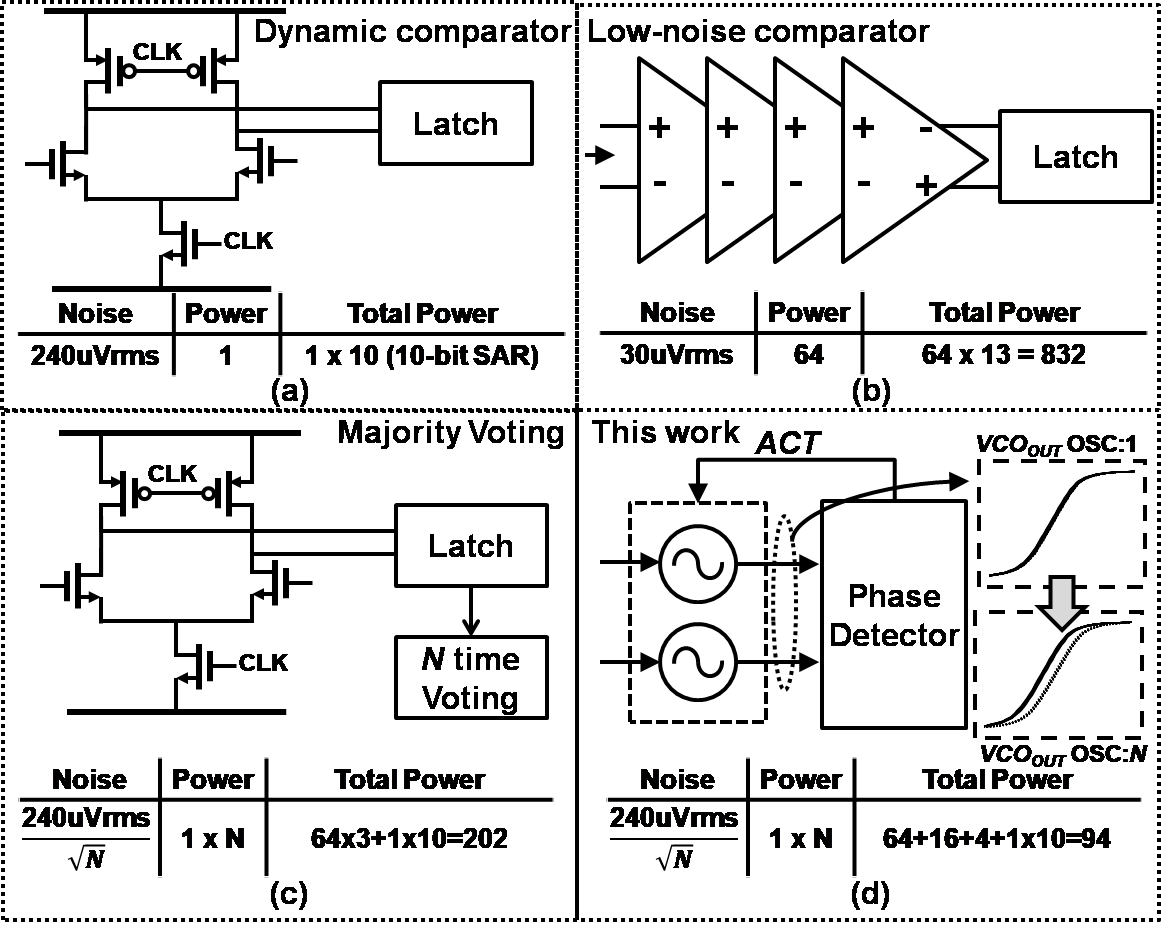
\includegraphics[width=0.5\textwidth]{figs/fig1.png}
  \captionsetup{font=footnotesize}
  \caption{\textbf{ADC}}
  \label{fig1}
\end{figure}
\begin{figure}[ht!]
\centering
 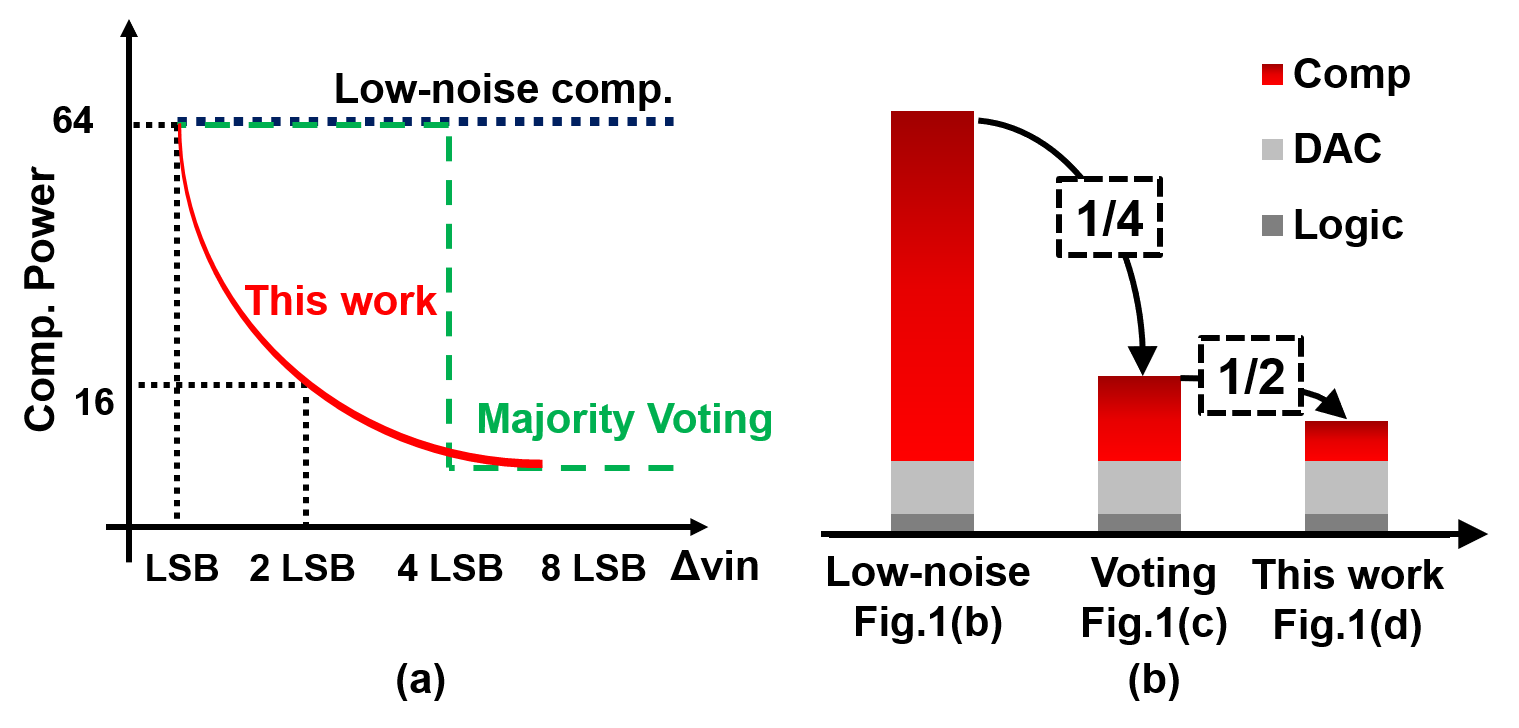
\includegraphics[width=0.5\textwidth]{figs/fig2.png}
  \captionsetup{font=footnotesize}
  \caption{\textbf{ADC}}
  \label{fig2}
\end{figure}
\begin{figure}[ht!]
\centering
 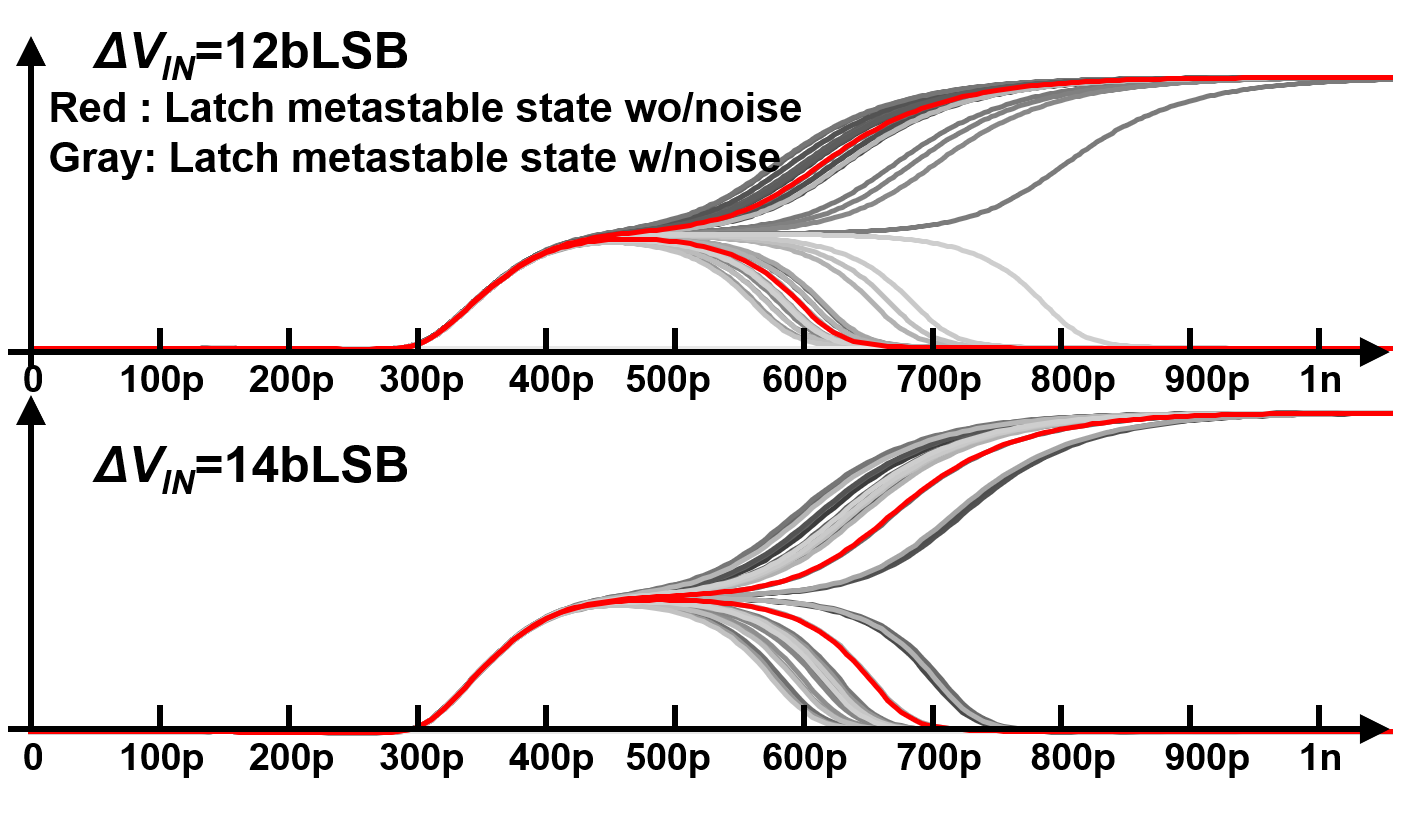
\includegraphics[width=0.5\textwidth]{figs/conventional-strongarm.png}
  \captionsetup{font=footnotesize}
  \caption{\textbf{ADC}}
  \label{meta}
\end{figure}

Fig.\ref{fig1}(a) shows a typical comparator\cite{miyahara2008low} used in low-power SAR ADCs. Although the noise can be reduced by limiting the bandwidth of the preamp stage, a typical design has an input referred noise (IRN) around 10b resolution. Fig.\ref{fig1}(b) shows a comparator used in 14b SAR ADC \cite{hesener200714b}: the comparator IRN is reduced by cascading preamp stages before the latch. However, during the successive approximation (SA) conversion, comparator input differential voltage ($\Delta V_{in}$) differs each cycle (Fig.\ref{fig2}(a)) Moreover, during the SA conversion, $\Delta V_{in}$ < LSB only occurs once, which is the situation when comparator noise requirement is most strict; the comparator noise requirement is relaxed at other cycles and utilizing a low-noise comparator for all of the cycles is inefficient. 

To cut down the comparator power, ref.\cite{harpe201310b} propose data-driven noise reduction (DDNR) technique, where the comparator triggers majority voting when the $\Delta V_{in}$ is sufficiently small for comparator meta-stability \cite{shikata20120}. The comparator output is decided given the result of $N$ time majority voting, and comparator IRN improves as:
\begin{eqnarray}
    \centering
    V_{noise_voting} = \frac{V_{noise}}{\sqrt{N}}
    \label{voting}
\end{eqnarray}

入力差が小さい時のみvotingを用いた低ノイズな比較器に切り替えることで変換時の比較器電力を大きく削減することができる。
Here, we conduct a simple analysis of the conversion comparator power of the conventional techniques. Ideally, to halve the comparator IRN, 4x much power is consumed. Therefore, when the power of the 10b resolution comparator is normalized as 1, the power of the 13b comparator can be described as:
\begin{eqnarray}
    \centering
    P_{13bcomp} = 1 \times 4^{13-10} = 64
    \label{13b}
\end{eqnarray}
Then, the total comparator power of 13b SAR ADC will be:
\begin{eqnarray}
    \centering
    P_{total(Fig.1(b)} = 64 \times 13 = 832
    \label{sar13b}
\end{eqnarray}
Next, we will assume an ideal DDNR done by 10b comparator, where majority voting is triggered when $\Delta V_{in}$ is smaller than 4LSB (corresponding to 11b resolution).
\begin{eqnarray}
    \centering
    P_{total(Fig.1(c)} = 64 \times 3 + 1 \times 10 = 202
    \label{ddnr}
\end{eqnarray}
The analysis shows that comparator power can reduced by over 1/4 with DDNR. $\Delta V_{in}$ versus comparator power is shown in Fig.\ref{fig2}(b), where the power of the majority voting is plotted in the dashed green line. 

DDNRは入力に応じて比較器のノイズ性能を切り替えることで、速度と引き換えに大きく比較電力を減らせることを示した。
一方でDDNRの比較器は2つしかノイズ性能を切り替えられず、結果として $\Delta V_{in}$ = 4LSBを超えると一気に消費電力が跳ね上がってしまう。例えば入力が4LSB相当であれば比較器のノイズ性能も4LSB相当で良く、 比較器のノイズ性能を入力レベルに応じ\textit{オンデマンド}で切り替えられれば更に比較エネルギーを低減することができる。 

比較器が入力電圧差を察知することができれば、DDNRのvoting回数を制御することでオンデマンドなノイズ性能を実現できる。
However, it is challenging for the 電圧ドメインのcomparator to detect the value of $\Delta V_{in}$ levels. Fig.\ref{fig2}(a))に10bノイズを持つ2-stage比較器\cite{miyahara2008low}に$\Delta V_{in}$を12bLSBと14bLSBを与えたときのラッチ応答を示す。ノイズがなければ(赤線)regeneration時間は$\Delta V_{in}$に比例する。一方でノイズを加えると、ノイズ影響で早期にラッチが開いてしまう場合も多く、regeneration時間から$\Delta V_{in}$のレベルを推定することはできず、$\Delta V_{in}$に応じた最適なVoting回数を定めるのは難しい。

我々は$\Delta V_{in}$に完全に適応し自動的にノイズ性能を設定可能なVCO比較器を提案する。理想的にはVCO比較器はFig.\ref{fig2}(b)に示す通り$\Delta V_{in}$に対し適応した比較エネルギーになるため、 the ideal VCO comparator power consumption can be calculated as:
\begin{eqnarray}
    \centering
    P_{total(Fig.1(d))} = 64+16+4+1\times 10=94
    \label{ddnr}
\end{eqnarray}
Ideally, this is half of that of the majority voting (Fig.\ref{fig2}(c)). 
具体的なVCO比較機の動作原理については次章に記述する。

%またTime domain comparators such as delay comparator \cite{agnes20089} はプロセススケーラビリティと低電力動作能力を持ち、発展が期待されている. 一方でこれらのnoise characteristics are not enough for high-resolution ADCs.

\section{VCO Comparator}
\subsection{VCO Comparator Fundamentals}
\begin{figure*}[ht!]
\centering
 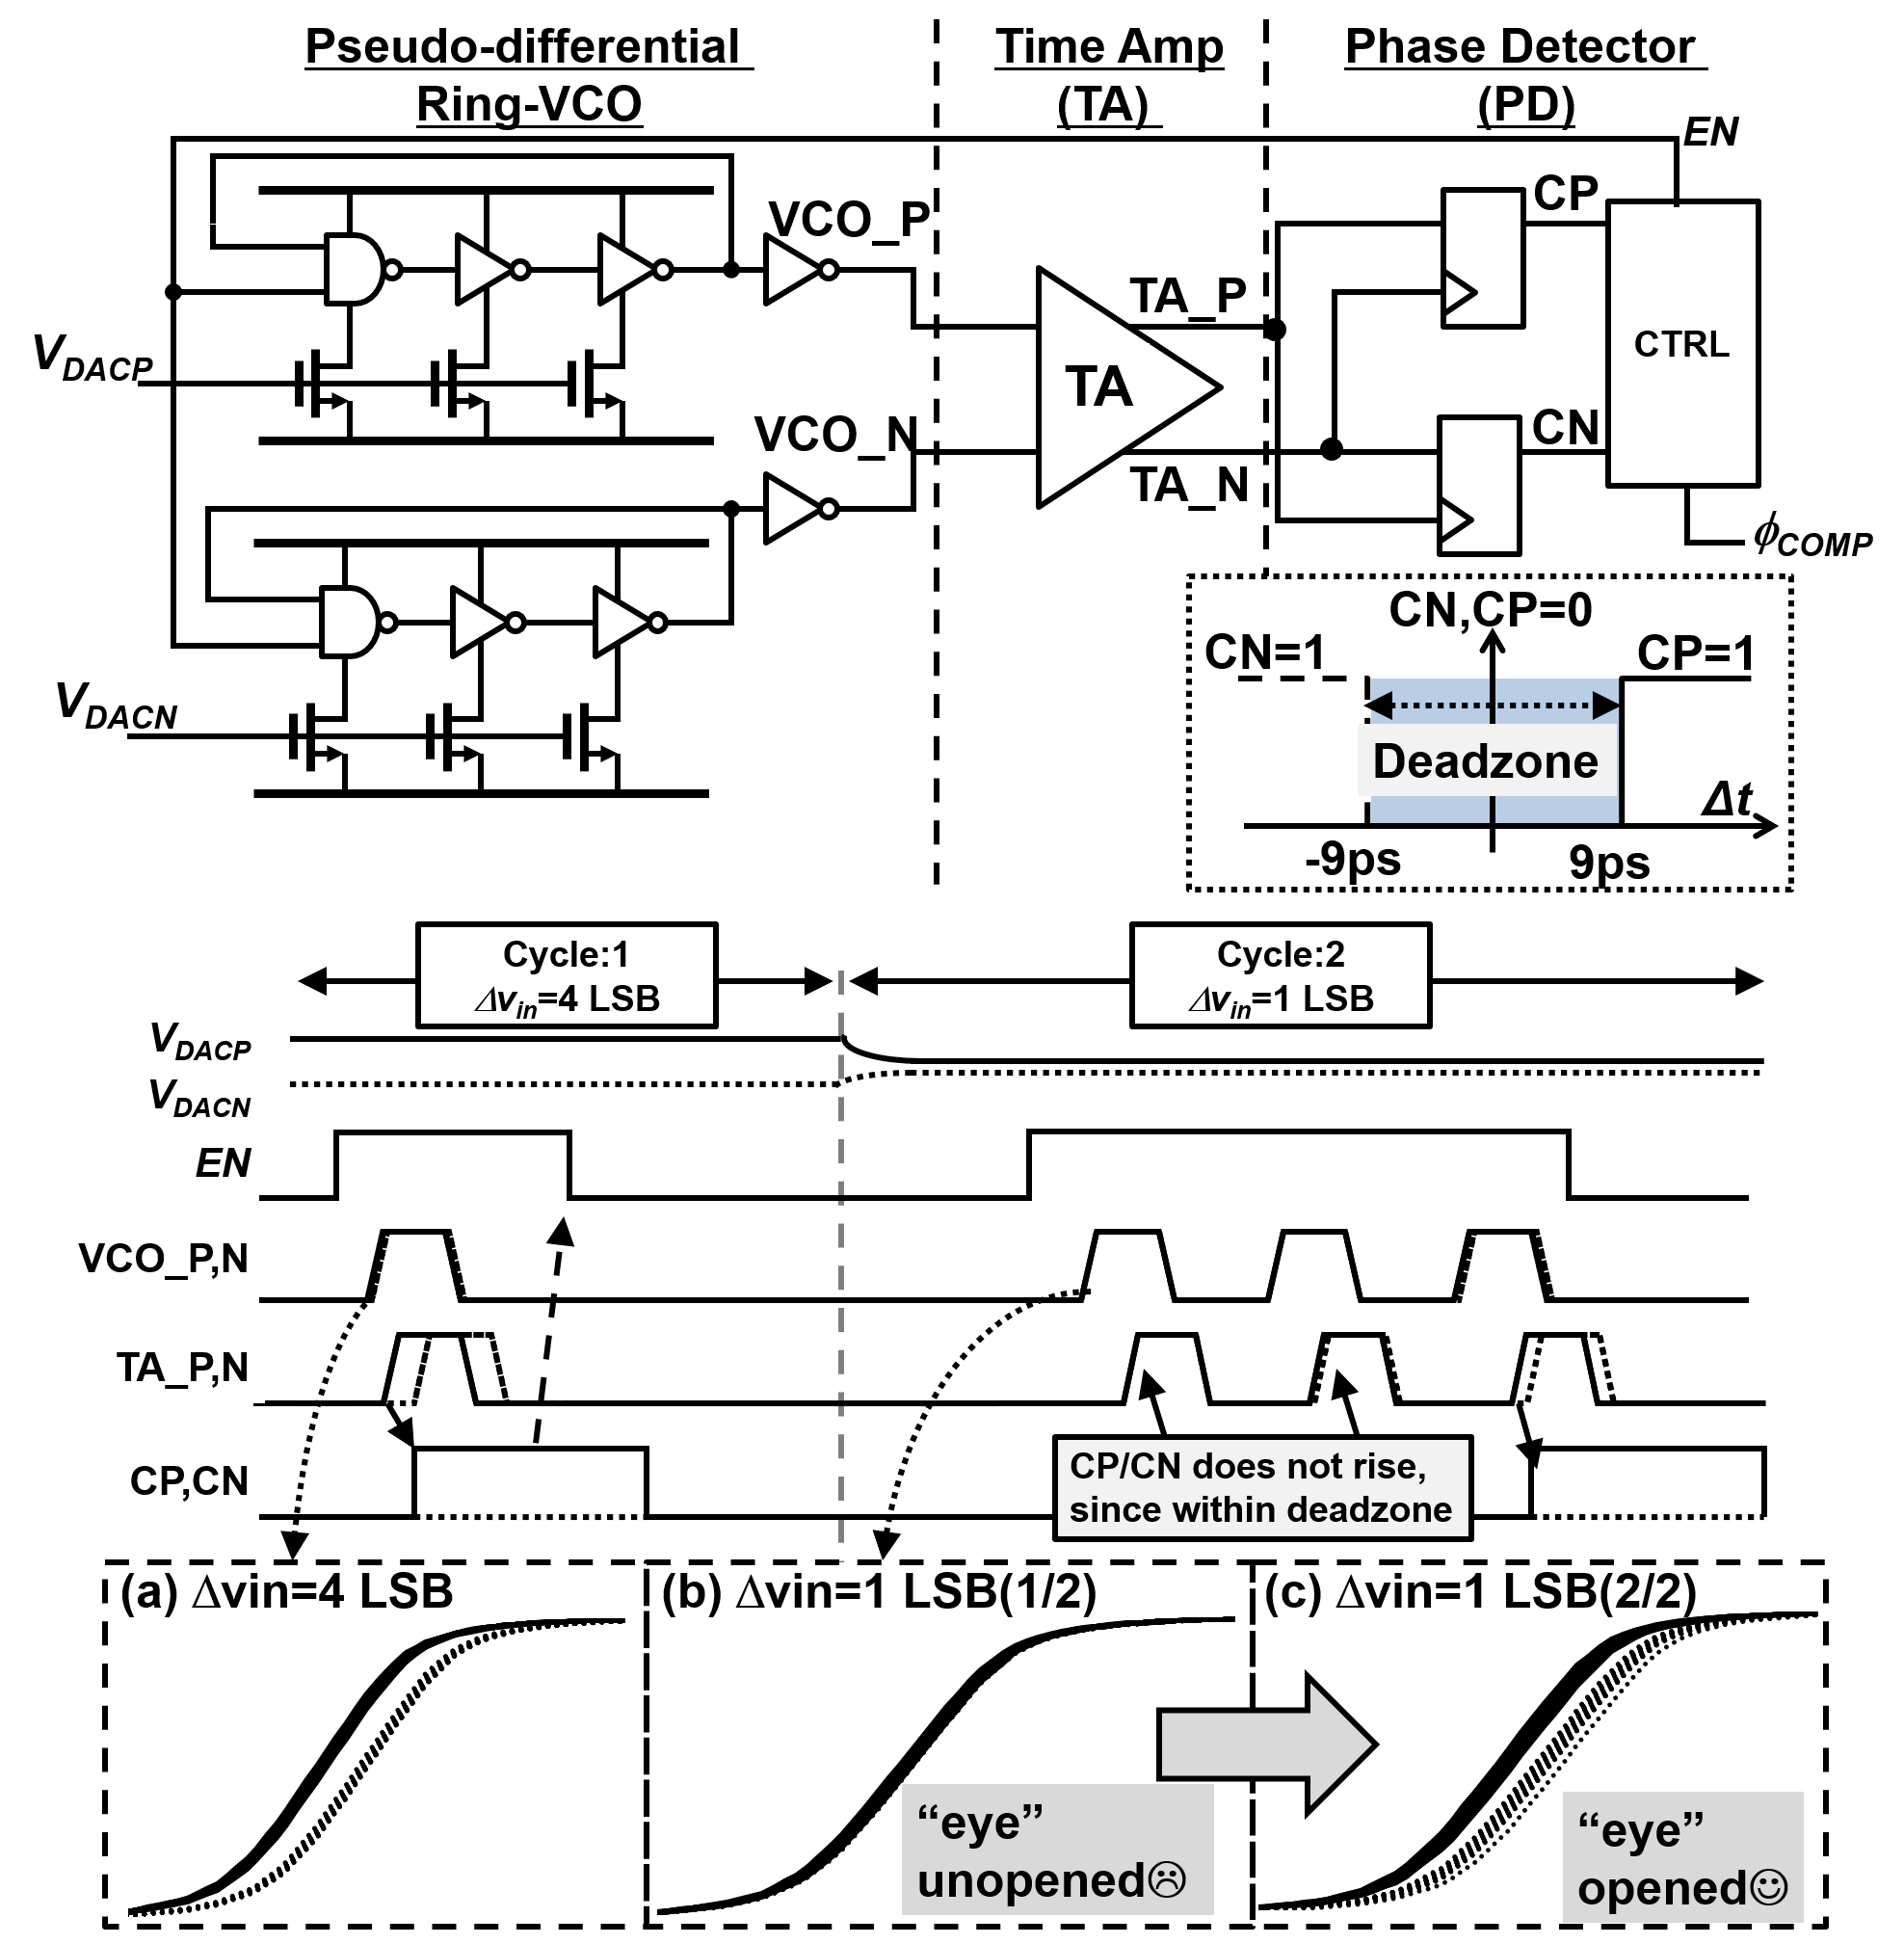
\includegraphics[width=0.9\textwidth]{figs/full.png}
  \captionsetup{font=footnotesize}
  \caption{\textbf{ADC}}
  \label{schema}
\end{figure*}

Fig.\ref{schema} shows the schematic of the VCO comparator. Similar to the delay line based comparators\cite{agnes20089}, the C-DAC analog voltages($V_{DACP}$, $V_{DACN}$) are given to control the slew rate (or the oscillating frequency) of the ring oscillator. We utilize a time amplifier (TA)\cite{lee20089} to amplify the “time” difference between the VCO outputs ($VCO_P$, $VCO_N$). Finally, the TA outputs ($TA_P$, $TA_N$) are connected to the phase detector, which resolves the comparison results.

Fig.\ref{schema}下部に shows the VCO comparator operation in the case of large and small $\Delta V_{in}$, respectively. In this example, at cycle 1, $\Delta V_{in}$ is fairly large (>4 LSB), and the VCO comparator operates as a delay line comparator. When $EN$ rises, the VCOs are "enabled" and pulses start to travel through the ring-VCO inverter cells. The pulses reach the TA and their time difference is amplified. In this case, $TA_P$ clearly rises faster than $TA_N$ and the D-FF based phase detector resolves the comparison results: CP=1 and CN=0. Once the comparison results are obtained, $EN$ is set down to “disable” the ring-VCO, which prevents unnecessary oscillations and resets the ring-VCO phase state.

Next, the comparator operation with small $\Delta V_{in}$ (Cycle 2 in Fig.\ref{schema}) is explained. Similarly, $EN$ rise and the pulses transmit through the VCOs. Fig.\ref{schema}(a) and (b) plot the VCO outputs of 50-times noise simulation with $\Delta V_{in}$ of 4 and 1 LSB, respectively. Note that in (b), an “eye” is not opened because the VCO jitter is larger than the input signal dependent time difference. In such conditions, the comparator cannot make a correct decision and noise reduction is required.

In VCO comparators, the event of small $\Delta V_{in}$ is detected by utilizing the $deadzone$ of the D-FF based PD. D-FF based phase detector (PD)はセットアップホールドが必要なため、入力時間差が短すぎると(<10ps)出力が反応しない有限のdeadzoneを持つことが知られている。
If the time difference of pulses is small and within the deadzone, the phase detector does not generate any output signal. Interestingly, since the VCOs are “enabled” during these events, the VCO consequently enters the second oscillation cycle and the oscillation (or signal integration) continues until the time difference is large enough to exceed the deadzone.
%これらのdeadzoneはPLL設計については特性悪化につながるため問題となるが、VCO比較機はdeadzoneを有効活用することでノイズ性能を入力差にフィットした値に設定する。
In Fig.4, the TA output exceeds the deadzone after 3 oscillations and comparison results are obtained and $EN$ set down. Fig.4(c) shows the noise simulation of VCO output after 3 oscillations and “eye-opening” is clearly observed. By this eye-opening oscillation, the VCO comparator adaptively reduces noise reflecting the level of $\delta V_{in}$.

\begin{figure}[ht!]
\centering
 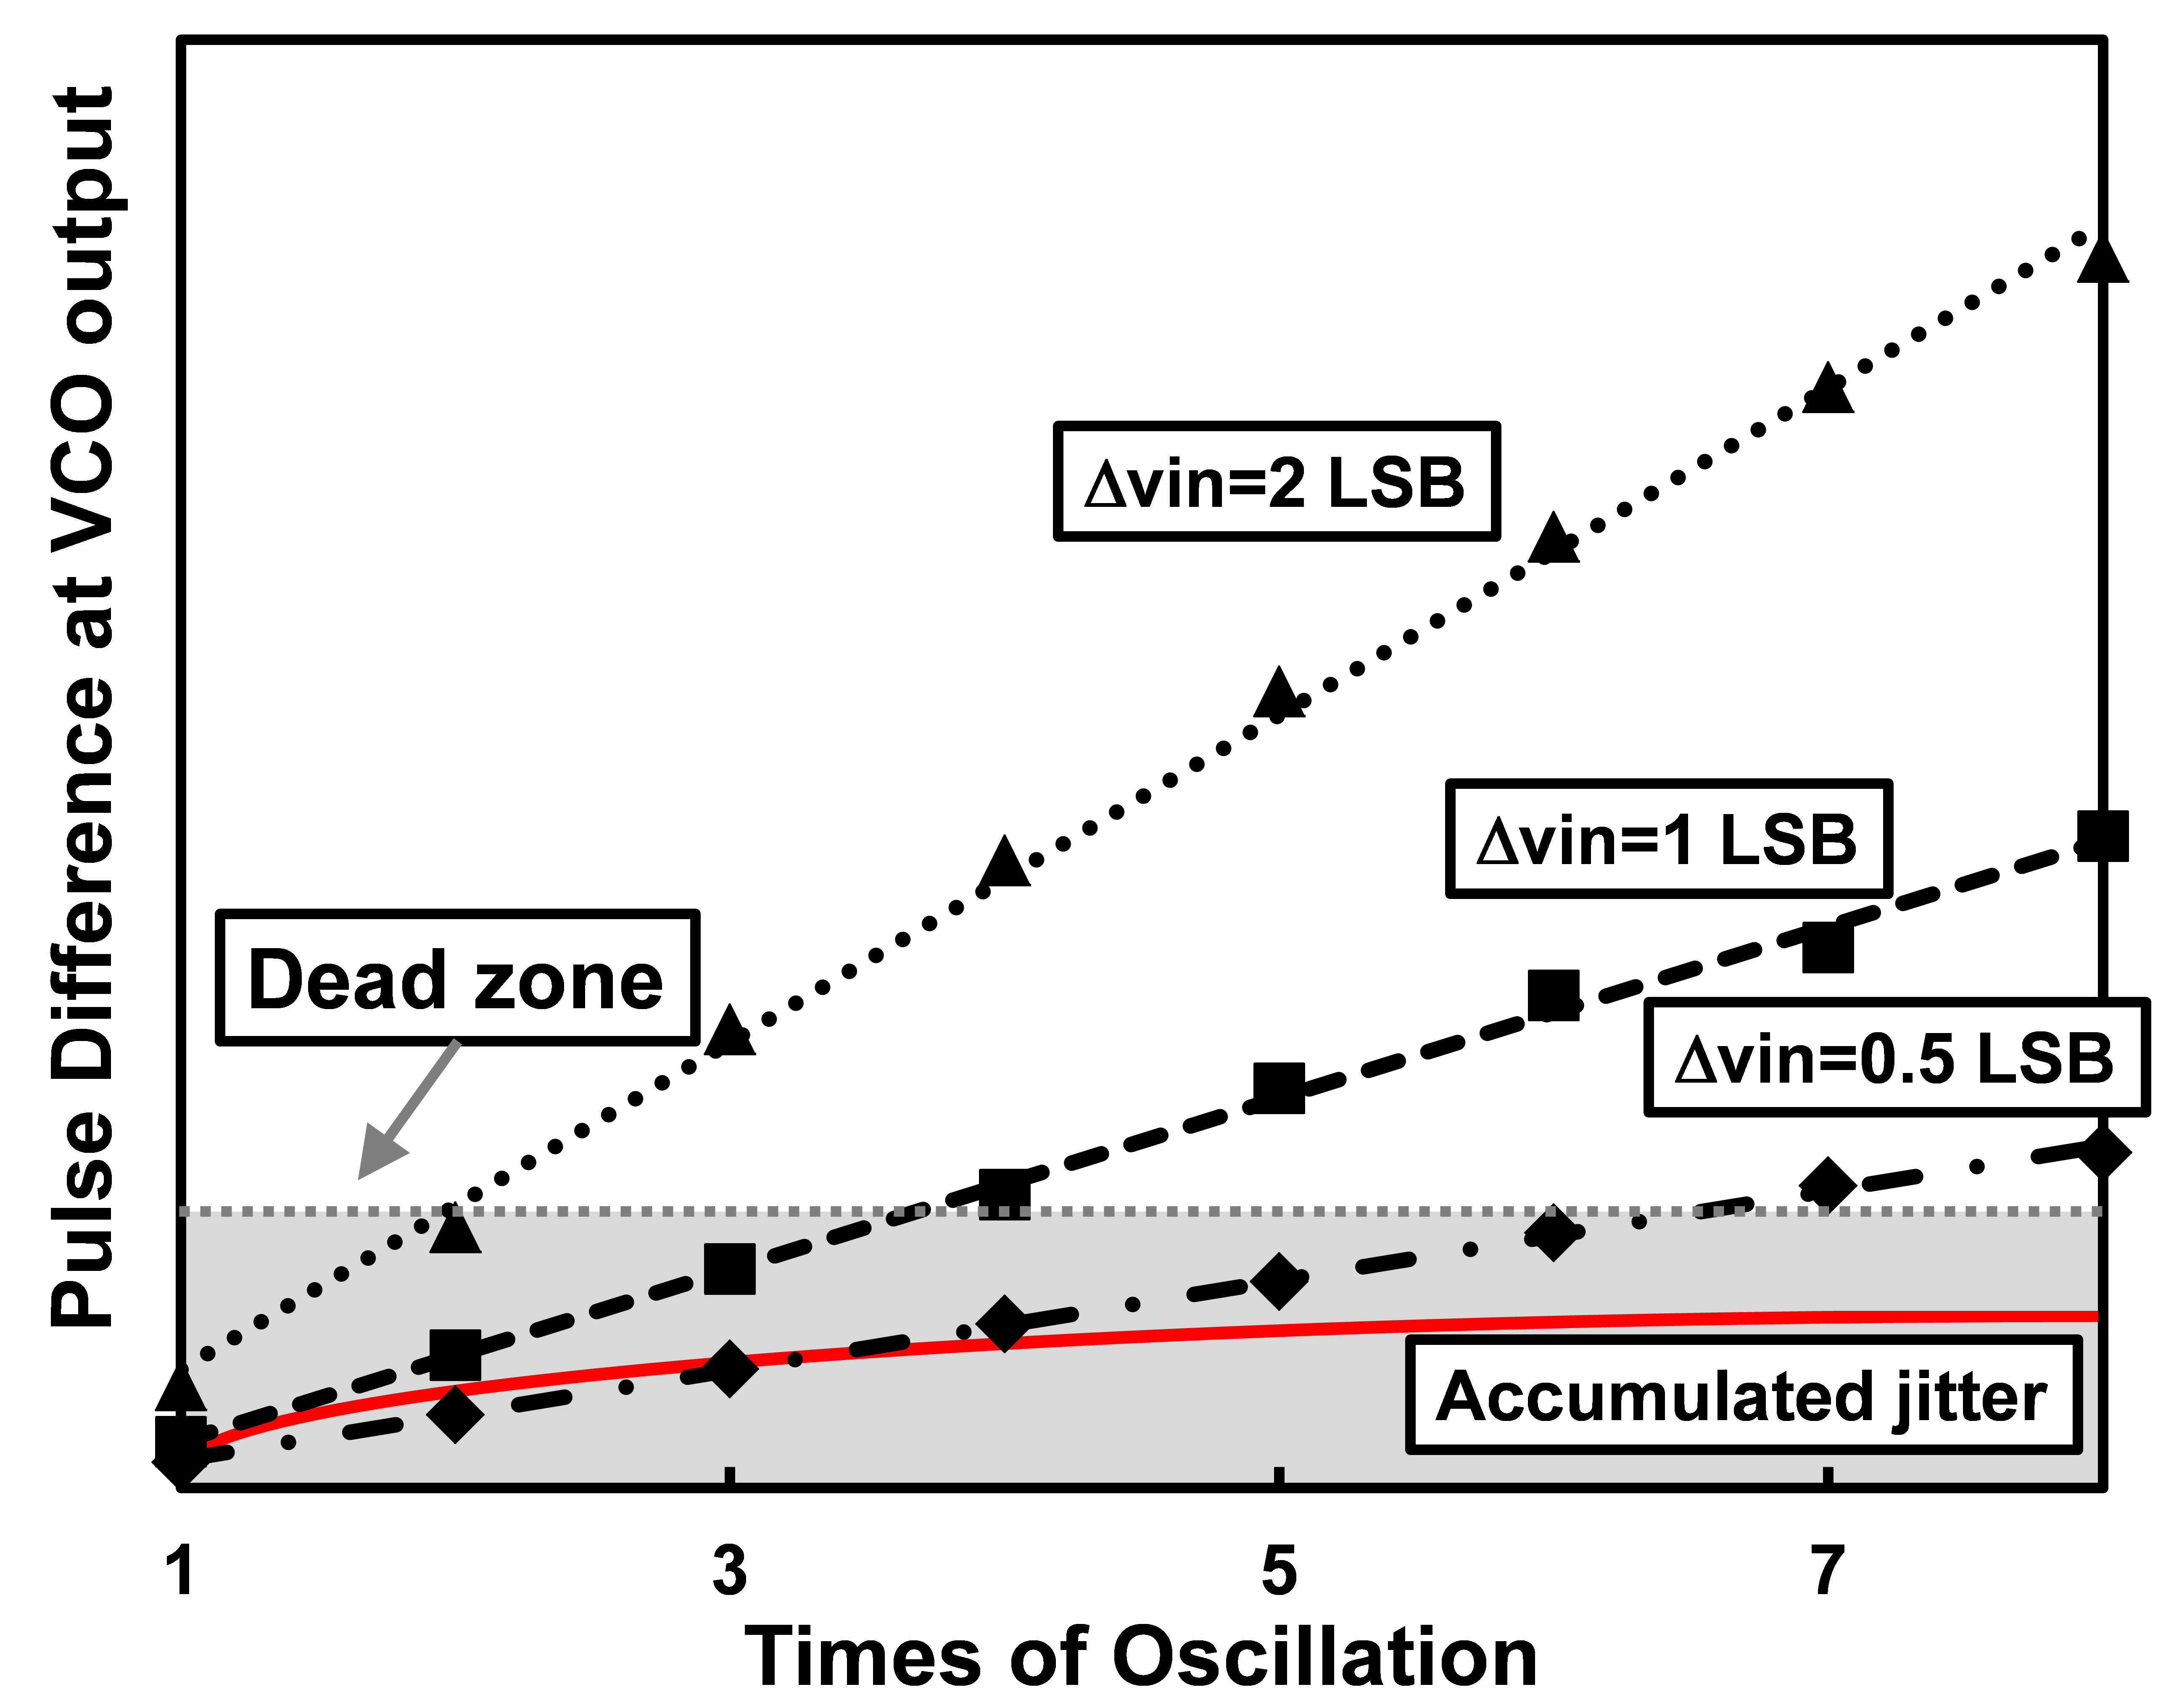
\includegraphics[width=0.5\textwidth]{figs/fig5.png}
  \captionsetup{font=footnotesize}
  \caption{\textbf{ADC}}
  \label{fig5}
\end{figure}

In Fig.5, the simulated eye-opening oscillation is given. In Fig.5, the simulation result of the Number of Oscillations ($N$) vs pulse difference is plotted for $\Delta V_{in}$ of 11b, 12b, and 13b LSB, respectively. We can observe that the oscillation times and pulse difference have a linear relationship of $\alpha N$ and $\alpha$ is decided by the $K_{VCO}$ and $\Delta V_{in}$. On the other hand, the accumulated jitter is proportional to $\sqrt N$\cite{hajimiri1999jitter,abidi2006phase}. In the case of $\Delta V_{in}$ of 13b LSB, even though the jitter may be dominant at 1-3 times of oscillation, the signal-dependent pulse difference will overcome the jitter as $N$ increase. The area in gray indicates the deadzone: as long as the pulse difference is within the deadzone, the oscillation will continue. Therefore, by careful design of the deadzone, VCO jitter, and $K_{VCO}$, we can design VCO comparators with the desired noise performance.

\subsection{Noise design guide of VCO comparators}
高精度比較器の設計に最も重要なのはノイズ設計であり、本節ではVCO比較器のノイズ設計指針について議論を行う。
VCO比較器のノイズ解析についてはref.\cite{luo2020input, ding20190}で詳細に述べられているものの、ノイズ設計指針については語られていない。
所望ノイズを満足するVCO比較器を設計するには大きく2つのステップを経る。
\begin{itemize}
\item 1. まずVCOブロックをある速度、ノイズを満足するdelay lineベース比較器として設計する。
ここで高精度な比較はeye-opening動作により実現できるため、この時のdelay lineベース比較器のノイズは必要とされる最高IRNの4-6倍程度で良い。
\item 2. そして最高ノイズ性能を引き出すためにTAのゲインによりVCOからみたデッドゾーンをチューニングする。
\end{itemize}

まずはVCOブロックをあるノイズを満足するdelay lineベース比較器として設計する。
単位遅延ステージの1サイクルのジッタはref.\cite{timecomp}より:
\begin{eqnarray}
    \centering
    jitter_{unit} = \frac{\sqrt{C_L\alpha k \rm{T}}}{I_{DS}}
    \label{ddnr}
\end{eqnarray}
ここでwhere α is the product of gm, output resistance ro, and noise factor γ and $I_{DS}$はインターた入力がVDD/2である時の引き抜き電流でk is Boltzmann’s constant.
また単位ステージの電圧-時間変換ゲインもref.\cite{timecomp}より:
\begin{eqnarray}
    \centering
    \rm{Gain} = \frac{g_mC_LV_{DD}}{2I_{DS}^2}
    \label{ddnr}
\end{eqnarray}
すると$N_{inv}$ステージのdelay-lineベース比較器のIRN($IRN_{DL}$)は
\begin{eqnarray}
    \centering
    IRN_{DL} = \frac{\sqrt{jitter_{unit}}}{\rm{Gain}} = \frac{1}{\sqrt{N_{inv}C_L}}\frac{2I_{DS}\sqrt{2\alpha k\rm{T}}}{V_{DD}g_m}
    \label{delaylineIRN}
\end{eqnarray}
と求まる。

\begin{figure}[ht!]
\centering
 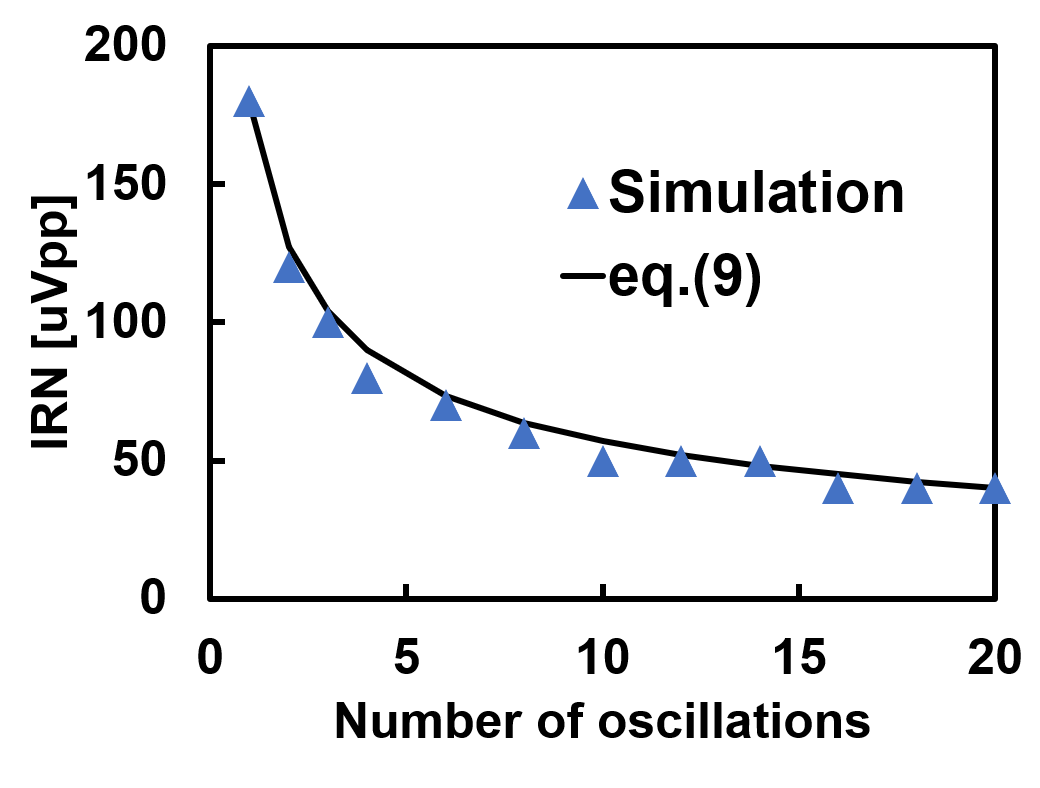
\includegraphics[width=0.4\textwidth]{figs/noc_noise.png}
  \captionsetup{font=footnotesize}
  \caption{Eq.(9)とノイズシミュレーションによって確認したVCO比較器ノイズの比較。ほぼeq.(9)に沿ったノイズ性能が得られることを確認できた。}
  \label{nocnoise}
\end{figure}

またfig.\ref{fig5}でも議論したとおりdelay lineをVCOに組み換え、発振動作をさせることで信号成分が積分されIRNが改善される。
発振回数を$N$とするとIRNは
\begin{eqnarray}
    \centering
    IRN_{VCO} = \frac{IRN_{DL}}{\sqrt{N}}
    \label{vcoIRN}
\end{eqnarray}
Fig.\ref{nocnoise}で\ref{vcoIRN}が成り立つことをtransient noise シミュレーションで確認した。発振回数=1における状態がdelay line比較器としての$IRN_{DL}$であり、発振回数のsquare rootのノイズ改善をシミュレーションでも確認することができた。

VCO比較器のadaptiveなノイズ性能を活かすためにはdelay lineベース比較器自体の電力は低ければ低いほどよい。経験則ではノイズ性能は得たい最高IRNの4倍程度悪化させ、出来るだけ低消費電力に設計すると全体比較器電力を最小化することができる。例えば\ref{delaylineIR}において入力トランジスタgmを最大化するように設計し、電力が増加する負荷、寄生容量を最小化するように務めるとよい。

% deadzoneの効果。VCOからみたdeadzoneはDFF deadzone/TA gain。
\begin{figure}[ht!]
\centering
 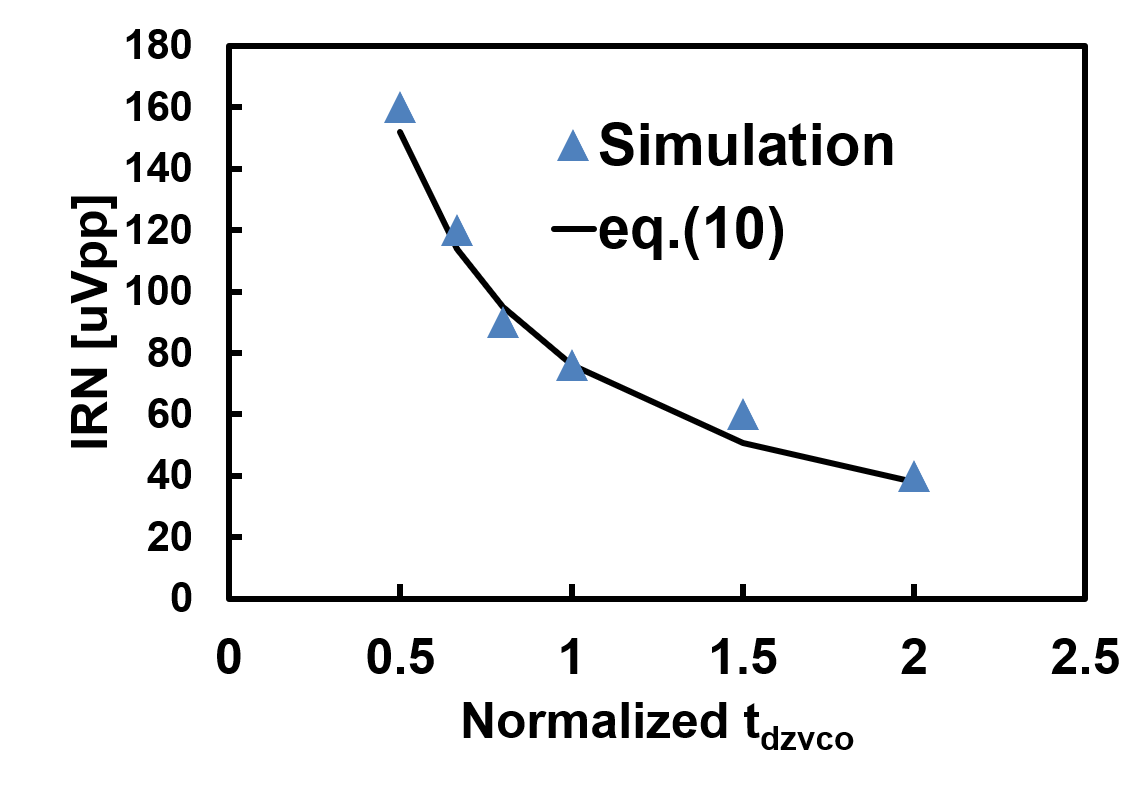
\includegraphics[width=0.4\textwidth]{figs/tdzvco.png}
  \captionsetup{font=footnotesize}
  \caption{tdzvco vs IRN。}
  \label{tdzvco}
\end{figure}

次にVCOから見えるdeadzoneを調整することでeye-opening動作を行うVCO比較器のノイズを設計する。
まず本回路はtime amplifierを備えるため、VCO出力から見たdeadzone($t_{dzvco}$)はTAのゲイン$G_{TA}$により圧縮され、
\begin{eqnarray}
    \centering
    t_{dzvco} = \frac{t_{dz}}{G_{TA}}
    \label{dzvco}
\end{eqnarray}
となる。そしてにref.\cite{luo2020input, ding20190}で議論されている通りVCO比較器のIRNはdeadzoneに反比例するため、\ref{dzvco}より:
\begin{eqnarray}
    \centering
    IRN \propto \frac{IRN_{DL}}{t_{dzvco}} = \frac{IRN_{DL}\times G_{TA}}{t_{dz}}
    \label{irn}
\end{eqnarray}
興味深いこと$G_{TA}$をチューニングすることで直接VCO比較器のIRNをチューニングできる。$t_{dz}$はセットアップホールドのため調整は難しく、$IRN_DL$の調整は比較器消費電力のインパクトが大きい。一方で$G_{TA}$は次章で詳しく述べる通り負荷容量の値で簡単に調整できVCO比較器ノイズ設計に大きな柔軟性をもたらす。Eq.(\ref{irn})を確認するため、transient noise simulationでTAゲインを調整しVCO比較器の$t_{dzvco}$をスイープしIRNを計測した結果をfig.\ref{tdzvco}に示す。ほぼeq.\ref{irn}通りのIRNが得られることがわかる。
また実際の$IRN$にはTAとPDのノイズも加算される。我々の設計ではTA、PDのノイズを合算しても$IRN$の1/4程度であったため、\ref{irn}から大きな乖離はない。

%\subsection{Power Saving Characteristics}
%提案したVCO比較器は入力レベルに応じたエネルギーを消費する。まず特性を確認するため、入力差を振ったシミュレーション結果のVdi%f vs Energyをプロット。
%VCO比較器はノイズをかんたんにプログラム可能。上記IRNは理論限界
%10, 10.5, 11, 11.5, 12, 12.5, 13, 13.5
%low noise vs ddnr vs vco comp.

\subsection{PVT drift resistance}

%\begin{table}[ht!]
%\centering
%\caption{}
%\label{tab:my-table}
%%\resizebox{width=0.4\textwidth}{!}{%
%\begin{tabular}{|l|l|l|l|}
%\hline
%              & TT/27℃ & SS/-40℃ & FF/125℃ \\ \hline
%GTA           & 8      & 10      & 6.3     \\ \hline
%%tdz           & 7.5    & 7       & 7.5     \\ \hline
%tdzvco        & 0.93   & 0.7     & 1.2     \\ \hline
%IRN{[}uVpp{]} & 75     & 95      & 100     \\ \hline
%\end{tabular}%
%}
%\end{table}

高精度比較器で課題となるのはPVTばらつきによるノイズ変動である。一般的には電流と熱雑音が増加するFF高温条件で比較器ノイズは最大値を迎え、その条件のノイズを抑え込むために多大な苦労を強いる。
一方でVCO比較器はタイムアンプの$g_m$依存性を上手く利用することで、PVTばらつきによるノイズ増加をキャンセルすることができる。

式(\ref{irn})からFF高温では$IRN_{DL}$は通常比較器と同様にノイズ増加してしまい、$t_{dz}$のPVT依存性は小さい。
一方で$G_{TA}$は$g_m$に反比例するためFF高温条件ではゲインが小さくなる。するとVCOから見たデッドゾーンはeq.(\ref{dzvco}より小さくなるため、VCO比較器のIRNを改善する方向にシフトする。結果としてPVTばらつきが生じても$IRN_{DL}$と$G_{TA}$が打ち消し合い、ノイズ増加を抑えることが可能である。シミュレーションで求めたPVTばらつきにおけるVCO IRNを表に示す。ノイズ増加は最も厳しいFF高温条件でもTTに比べ30\%程度に抑えられる。

\subsection{Meta-stability detection}
高精度比較器は長いメタステーブル時間を持ち、非同期高精度SAR ADCにおいて変換エラーをもたらす危険性をはらむためメタステーブル検知機能は必須である。
従来比較器は比較時間をモニタすることでメタステーブル検知を行う場合が多いが、これはPVT依存性が大きくキャリブレーション等が必要となる\cite{shikata20120}。

一方でVCO比較器は本質的にメタステーブル状態の検知機能を備えPVTキャリブレーションも必要がない。VCO比較器のメタステーブル状態では理想的にはデッドゾーンから位相差が抜け出せないため、VCOは延々と発振を続ける。そのため単純に発振回数をカウントすることでメタステーブル検知が実現可能である。我々の設計ではカウンタ回路によってVCO発振回数をモニタし発振回数がX回を超えるとメタステーブルを検知し、ランダムな判定結果を格納する。このようなメタステーブル検知機能を活用することでadditional bit判定\cite{shikata20120,ding20190}やDACキャリブレーション\cite{zhu201914}をPVT依存性少なく実現可能である。

\section{Circuit Implementations}
\subsection{13-bit SAR ADC implementation}

\begin{figure*}[ht!]
\centering
 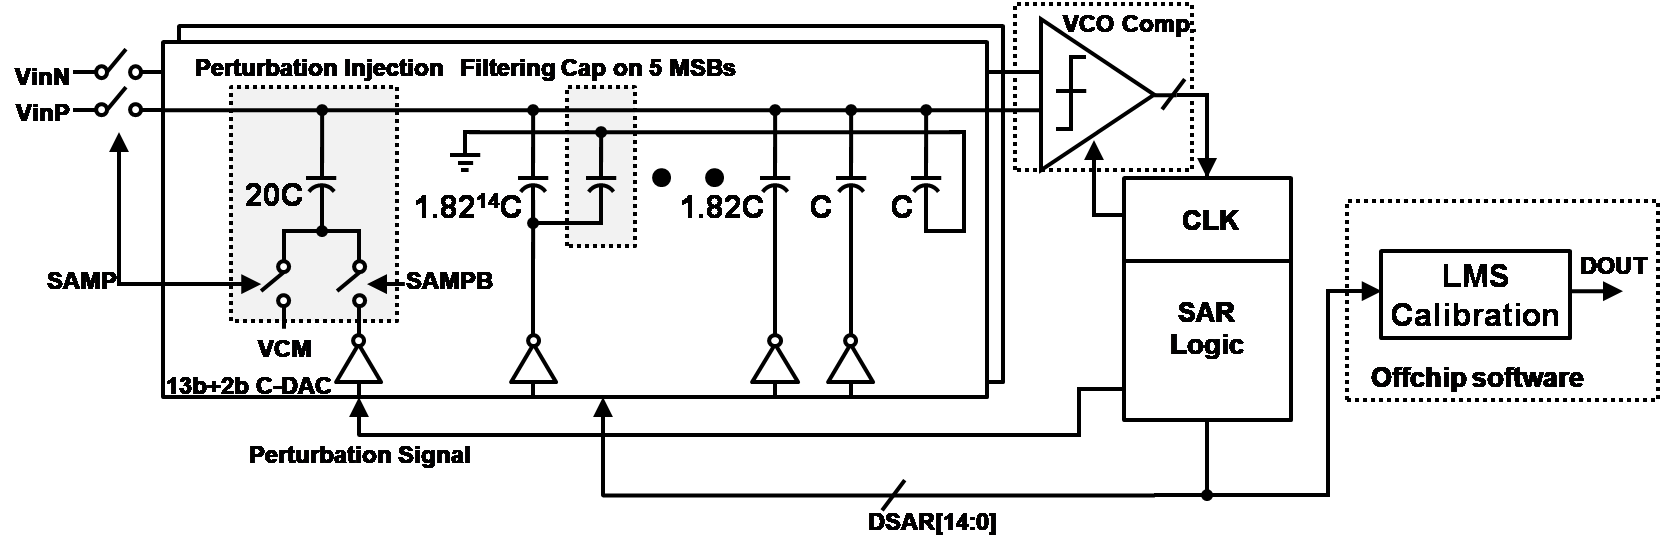
\includegraphics[width=1\textwidth]{figs/fig7.png}
  \captionsetup{font=footnotesize}
  \caption{\textbf{ADC}}
  \label{13bsar}
\end{figure*}

高精度なVCO比較器を実証するため、13bitの低電力SAR ADCを設計する。
The entire 13b SAR ADC architecture is shown in Fig.\ref{13bsar}. C-DACの電力をできるだけ低減するため、ref.\cite{liu201012b}と同様の sub-binary C-DAC and perturbation logic for LMS calibrationを用いる. The C-DAC has 2b redundancy and has a sub-binary radix of 213/15=1.82. To suppress the noise of C-DAC buffers, filtering capacitors \cite{miki20154} are provided until the 5th bit of MSB. Unit capacitor (C) of 0.5fF was chosen  to meet the kT/C noise requirements.

To cancel the capacitor mismatch effect, perturbation based digital calibration \cite{liu201012b} is employed. When the calibration is active, two conversions are resolved for a same sample. The conversions are perturbed with offset of $\pm \delta$ is injected before the SA cycle starts. The perturbation injecting capacitor is 20C as shown in Fig.\ref{13bsar}. After the first conversion ends, the perturbation signal is inverted so that it will inject with different polarity. In this work, the LMS calibration engine was implemented fully off-chip.

\subsection{VCO Comparator with multiple noise modes}
\begin{figure}[ht!]
\centering
 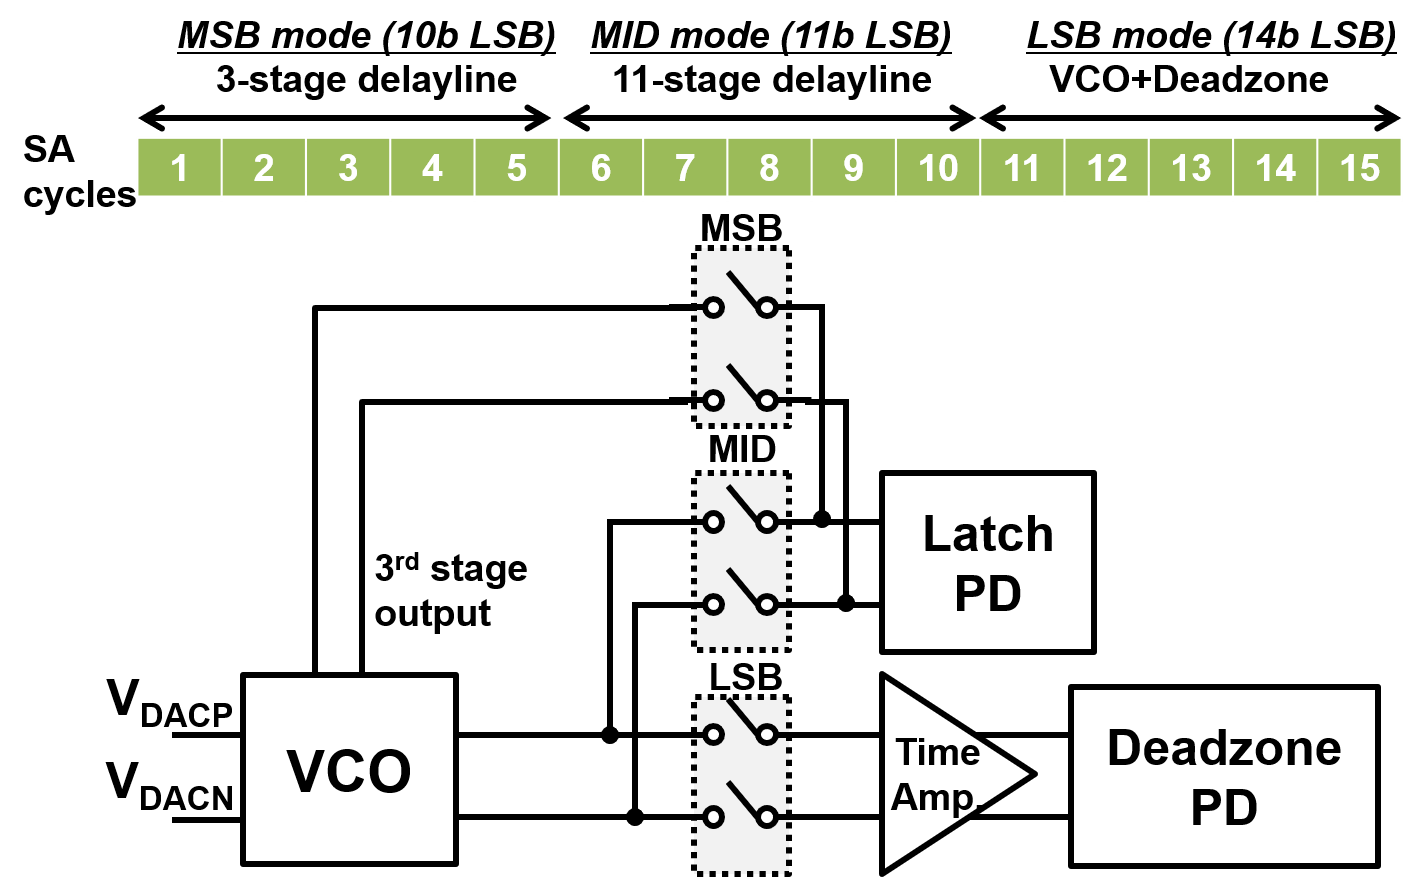
\includegraphics[width=0.5\textwidth]{figs/vco-entire-r1.png}
  \label{fullvco}
\end{figure}

高精度SAR ADCではセトリングなどの影響を緩和するため冗長性込で設計することが多い。
今回の13-bit SAR ADCもsub-binary radixであり2bitの冗長性をもたせている。
このような冗長性があるSAR ADCでは比較器入力が<LSBとなるのが一度だけとは限らない。更にbit毎に冗長性が割り当てられるため上位bitの判定エラーを下位bitが精微であればエラーコレクションすることができ全体としての精度を保証できることが知られている\cite{kapusta201314b}。例えば今回の設計では上位5bitでは200 LSB相当の判定エラーを許容でき、上位ビットにおいてsub-LSB精度を持つVCO comparatorを用いるのはエネルギーの無駄となる。

我々は複数のノイズ性能を可変にできるVCO比較器を提案する。(Fig.\ref{fullvco})
アイデアとしてはdelay line comparatorと発振を行うVCO比較器の動作を切り替えることでノイズパフォーマンスと消費電力をスケールすること。
少ない面積と簡単なスイッチング回路でVCO比較器に3つのノイズモードをもたせる。

\begin{itemize}
\item 上位5SA。MSBモード:単純な3-stage delay lineとして動作。判定エラーを許容できる上位比較。 IRN:2mVpp
\item 中間5 SA。MIDモード:11-stage delay lineとして動作。 IRN:180uVpp
\item 下位5SA。LSBモード:2章で記述した11-stage VCO動作。IRN:80uVpp
\end{itemize}

MSB,MidではDeadzoneを用いたPhaseDetectorで判定せず、ラッチベースのPhaseDetectorで強制的に判定結果を取得。

\subsection{Time Amp. designs}
\begin{figure}[ht!]
\centering
 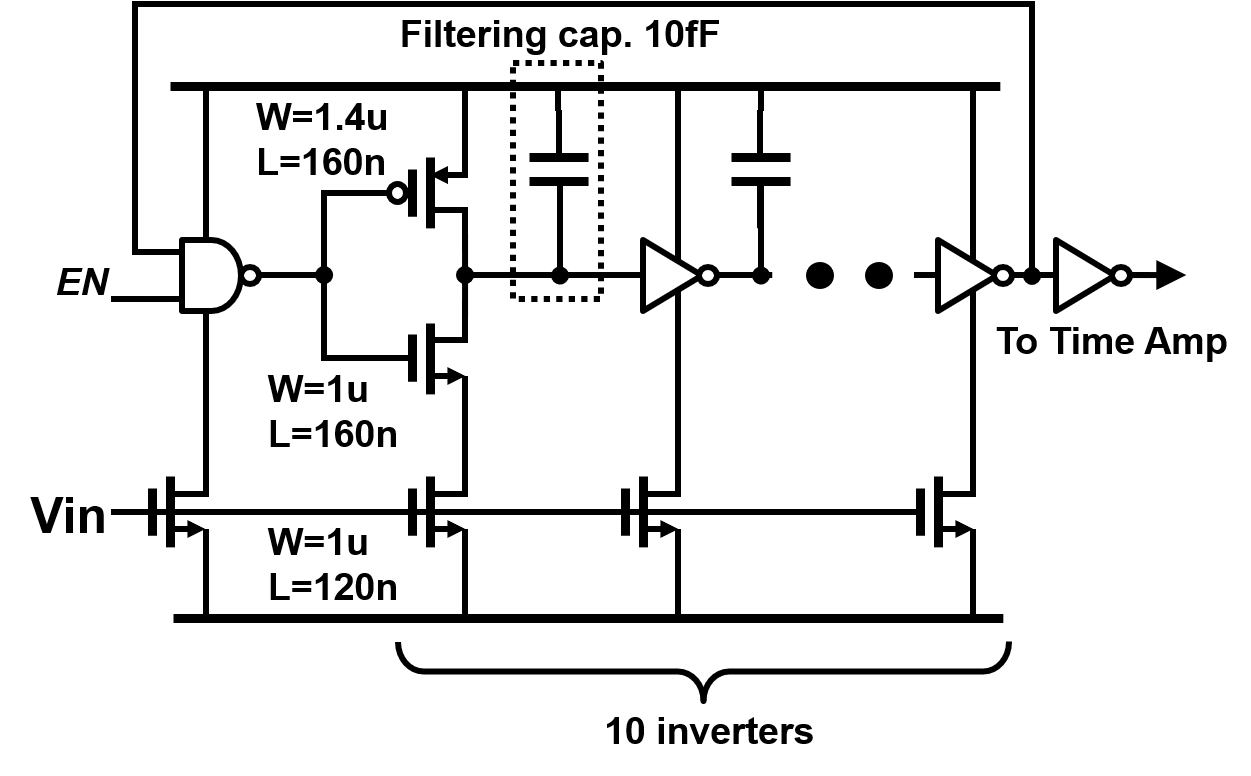
\includegraphics[width=0.5\textwidth]{figs/vco_cell.png}
  \captionsetup{font=footnotesize}
  \caption{\textbf{ADC}}
  \label{cell}
\end{figure}

\begin{figure}[ht!]
\centering
 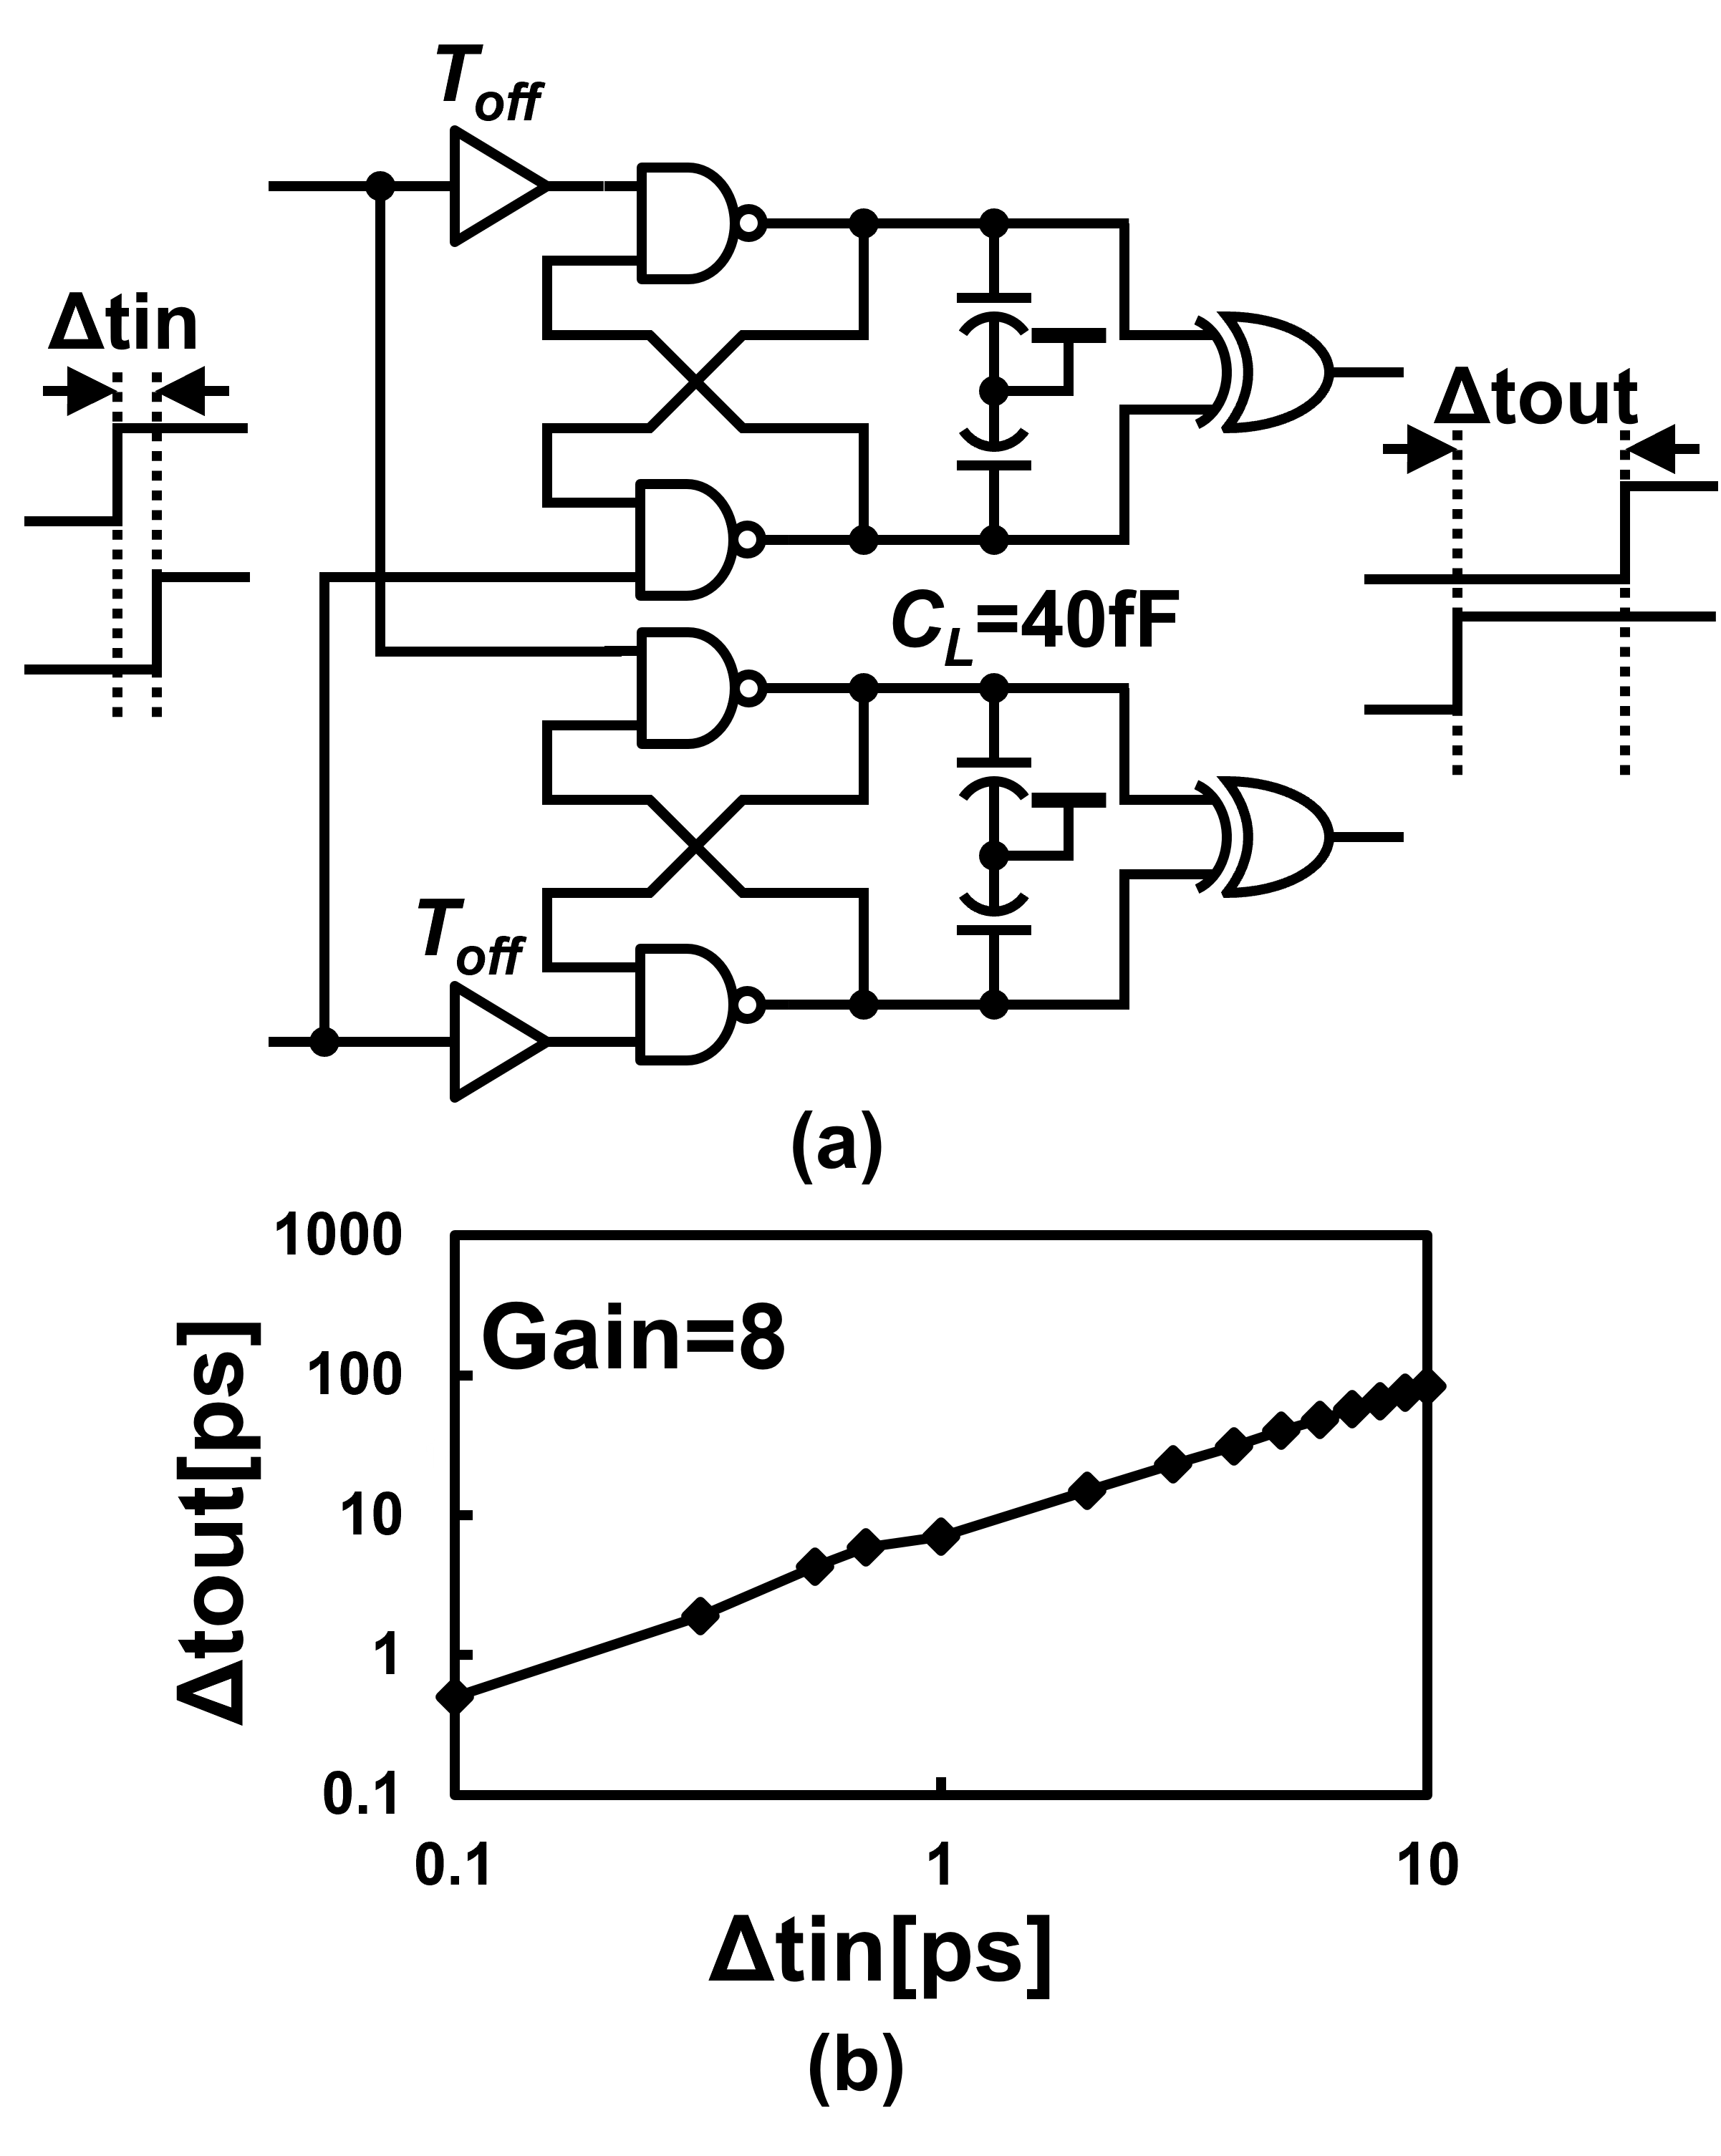
\includegraphics[width=0.5\textwidth]{figs/ta_chara.png}
  \captionsetup{font=footnotesize}
  \caption{\textbf{ADC}}
  \label{timeamp}
\end{figure}

最後にVCOセルとtime amplifierの設計について記述する。単位VCOセルはFig.\ref{cell}に示すとおり、インバータのNMOS側をcurrent-sturve形式で縛ることで電圧-時間変換を実現する。インバータステージ数はノイズと消費電力のバランスに優れる11ステージを選択した。また\cite{lee20089}のようにPMOS側の電流も縛ることでVCOの電圧ー時間変換ゲインを高め更にノイズ性能を消費電力の追加コスト少なく向上できる。しかしながらP側も縛ってしまうとVCOの発振周波数が大きく落ちてしまい、我々のターゲットとする1MS/s SAR ADC動作にはそぐわなかった。本設計のVCOはコモンモード電圧(500mV)が与えられたとき、600MHzで発振するように設計しており1MS/s SAR ADCの速度にも十分対応可能である。

Time amplifierはref.\cite{lee20089}にて提案された設計を結集しており、スケマをFig.\ref{timeamp}に示す。
$G_{TA}$は
\begin{eqnarray}
    \centering
    G_{TA} = \frac{2C_L}{g_mT_{off}}
    \label{gta}
\end{eqnarray}
と求められ\cite{lee20089}、前節で述べたとおりFF高温条件では$g_m$が増加するとゲインが減る方向に変化する。
今回の設計では$t_{off}$と負荷容量を調節しTTにおけるゲインが8となるように設計している。

% ここまで書いた
\section{Experiment Results}
\begin{figure}[ht!]
\centering
 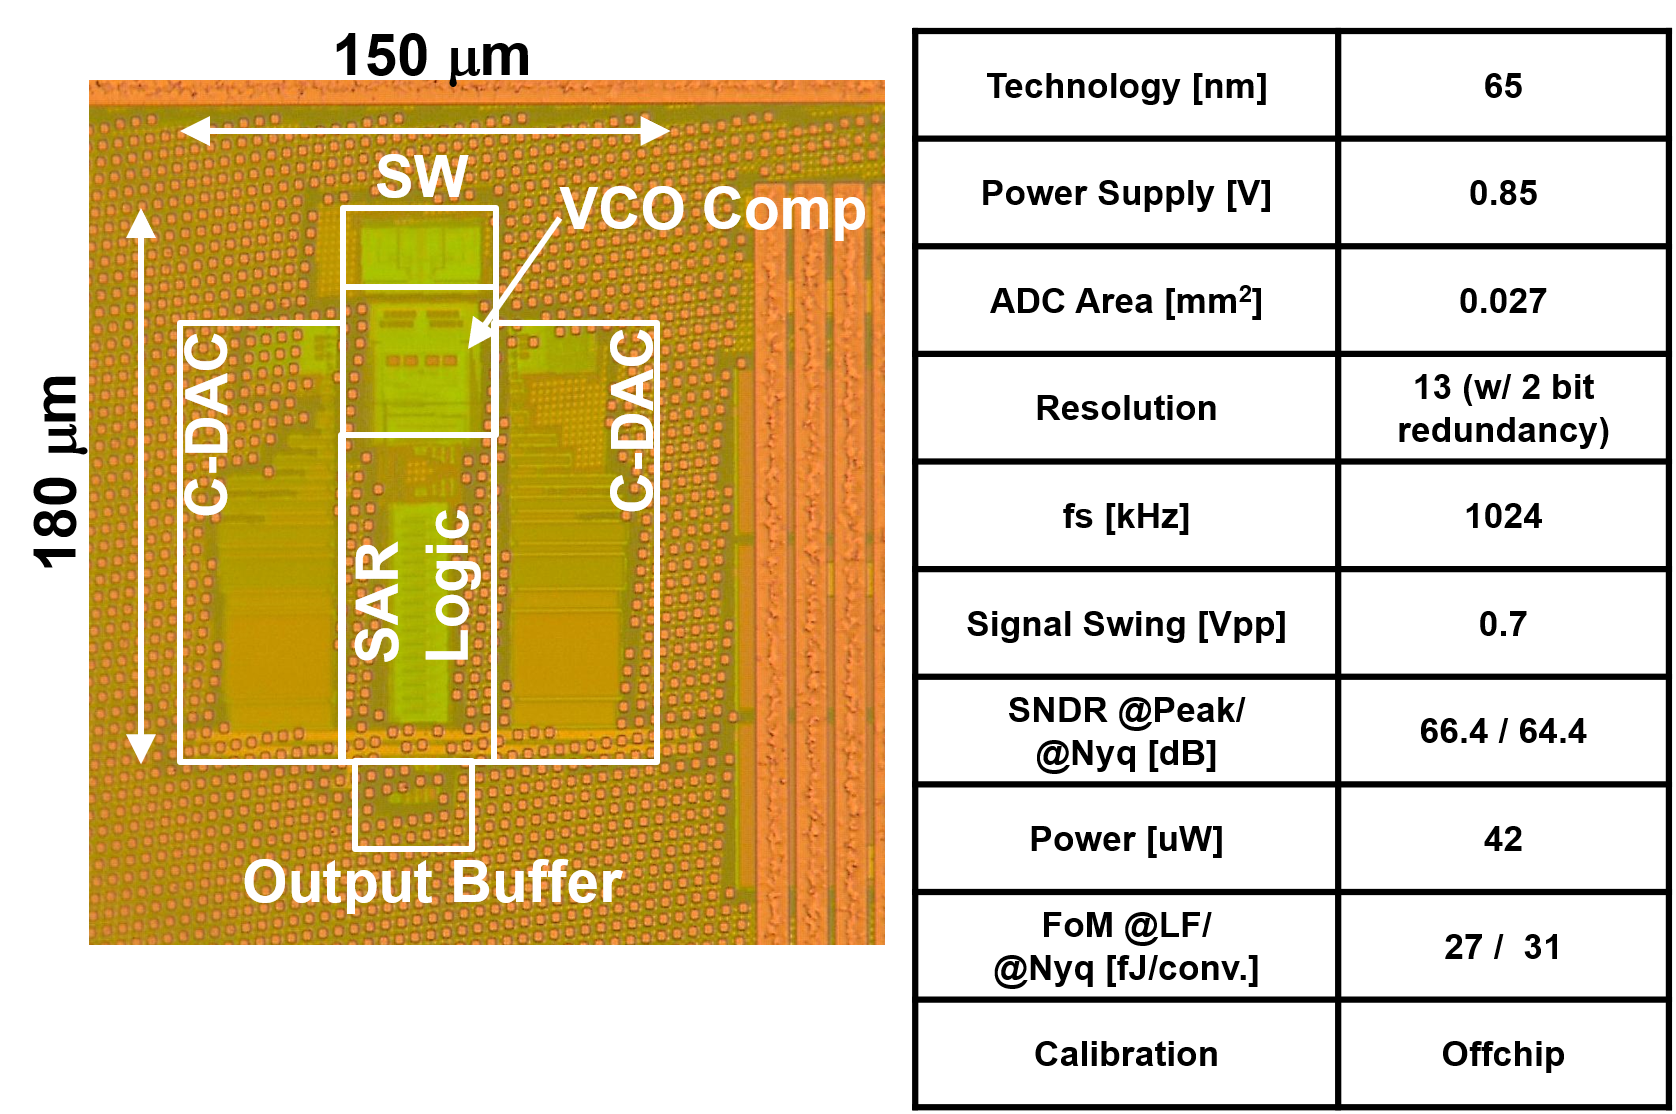
\includegraphics[width=0.5\textwidth]{figs/chipphoto.png}
  \captionsetup{font=footnotesize}
  \caption{\textbf{ADC}}
  \label{highlight}
\end{figure}

\begin{figure}[ht!]
\centering
 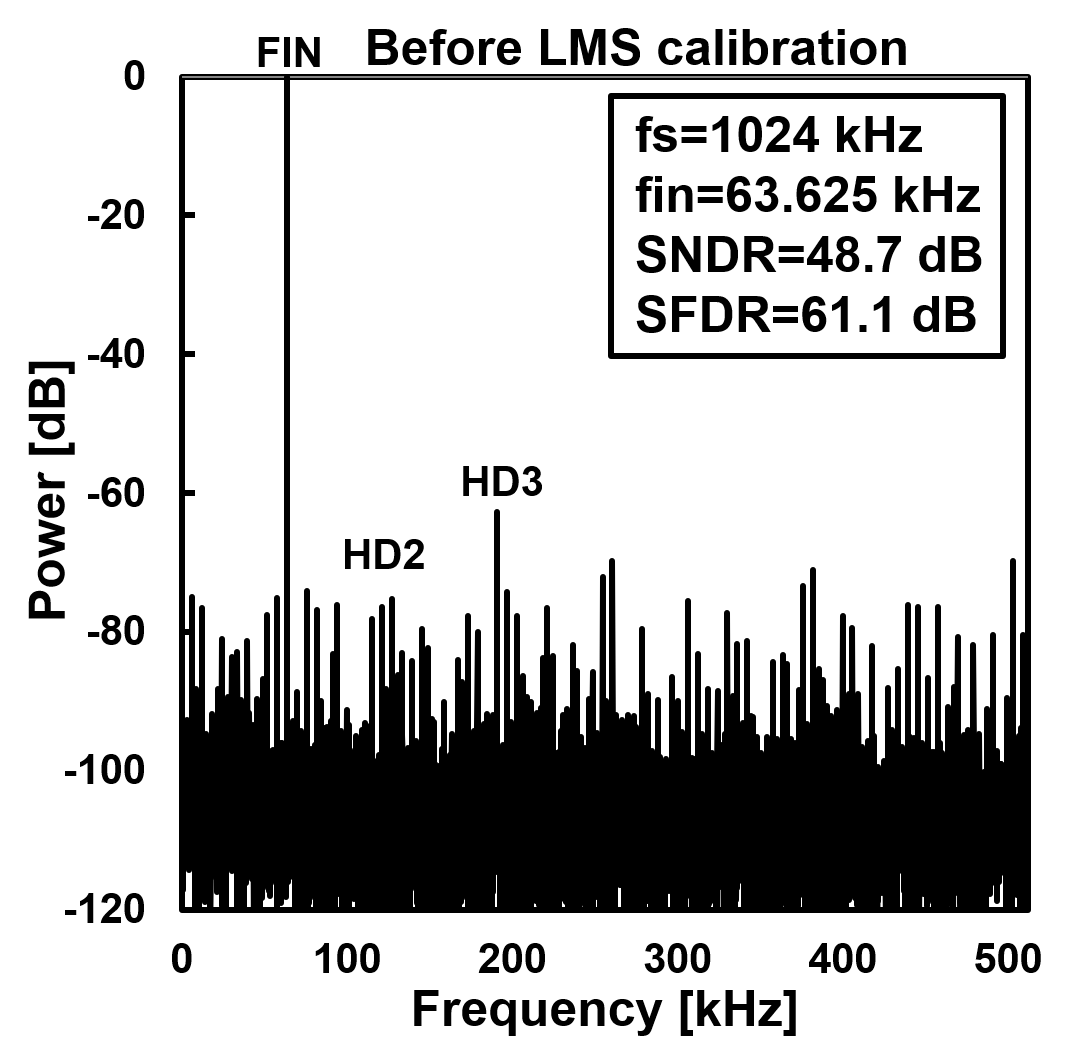
\includegraphics[width=0.5\textwidth]{figs/beforecal.png}
  \captionsetup{font=footnotesize}
  \caption{\textbf{ADC}}
  \label{highlight}
\end{figure}

\begin{figure}[ht!]
\centering
 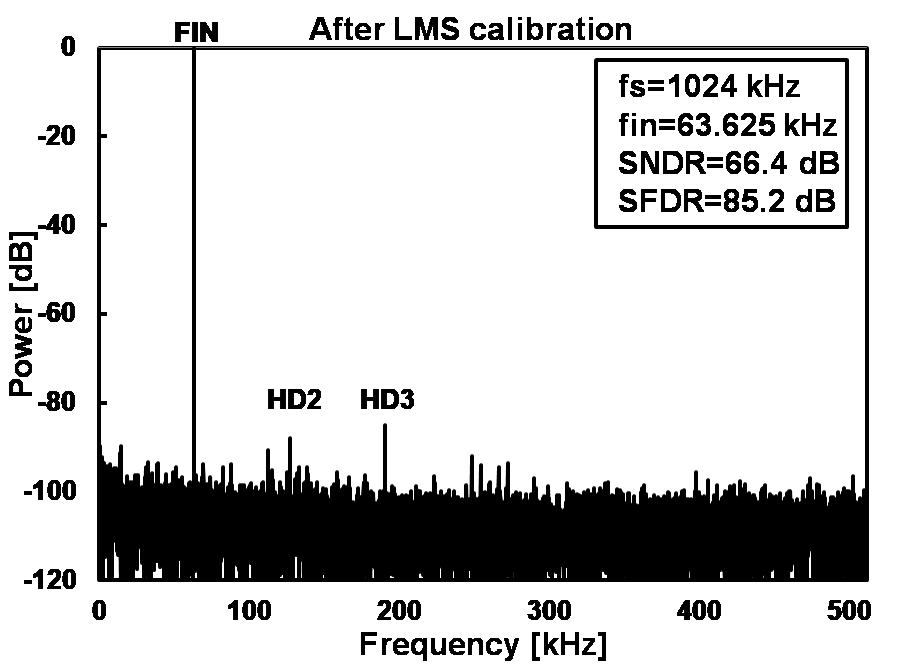
\includegraphics[width=0.5\textwidth]{figs/aftercal.png}
  \captionsetup{font=footnotesize}
  \caption{\textbf{ADC}}
  \label{highlight}
\end{figure}

\begin{figure}[ht!]
\centering
 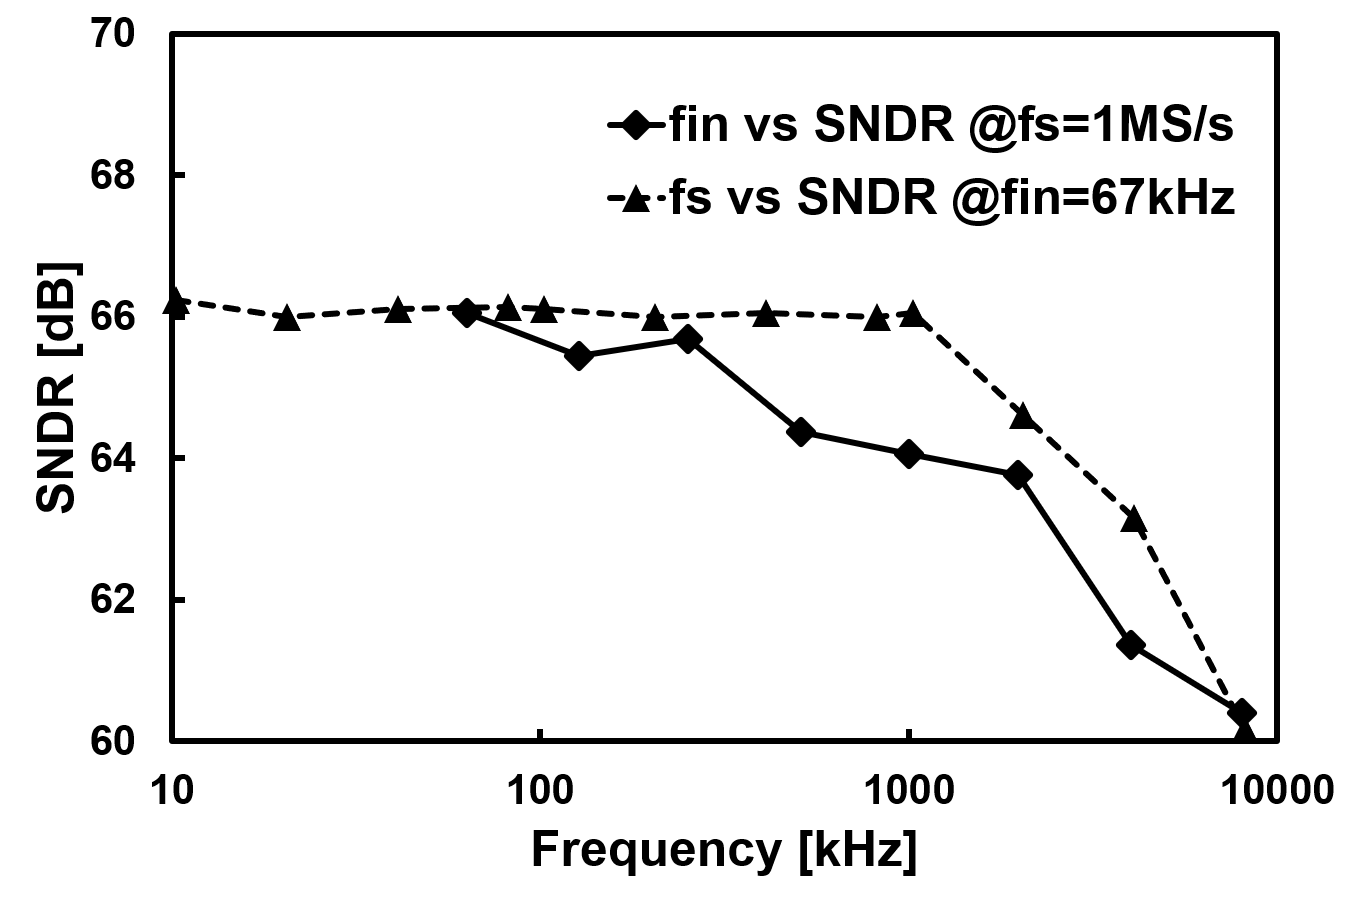
\includegraphics[width=0.5\textwidth]{figs/freq-sndr.png}
  \captionsetup{font=footnotesize}
  \caption{\textbf{ADC}}
  \label{highlight}
\end{figure}

\begin{figure}[ht!]
\centering
 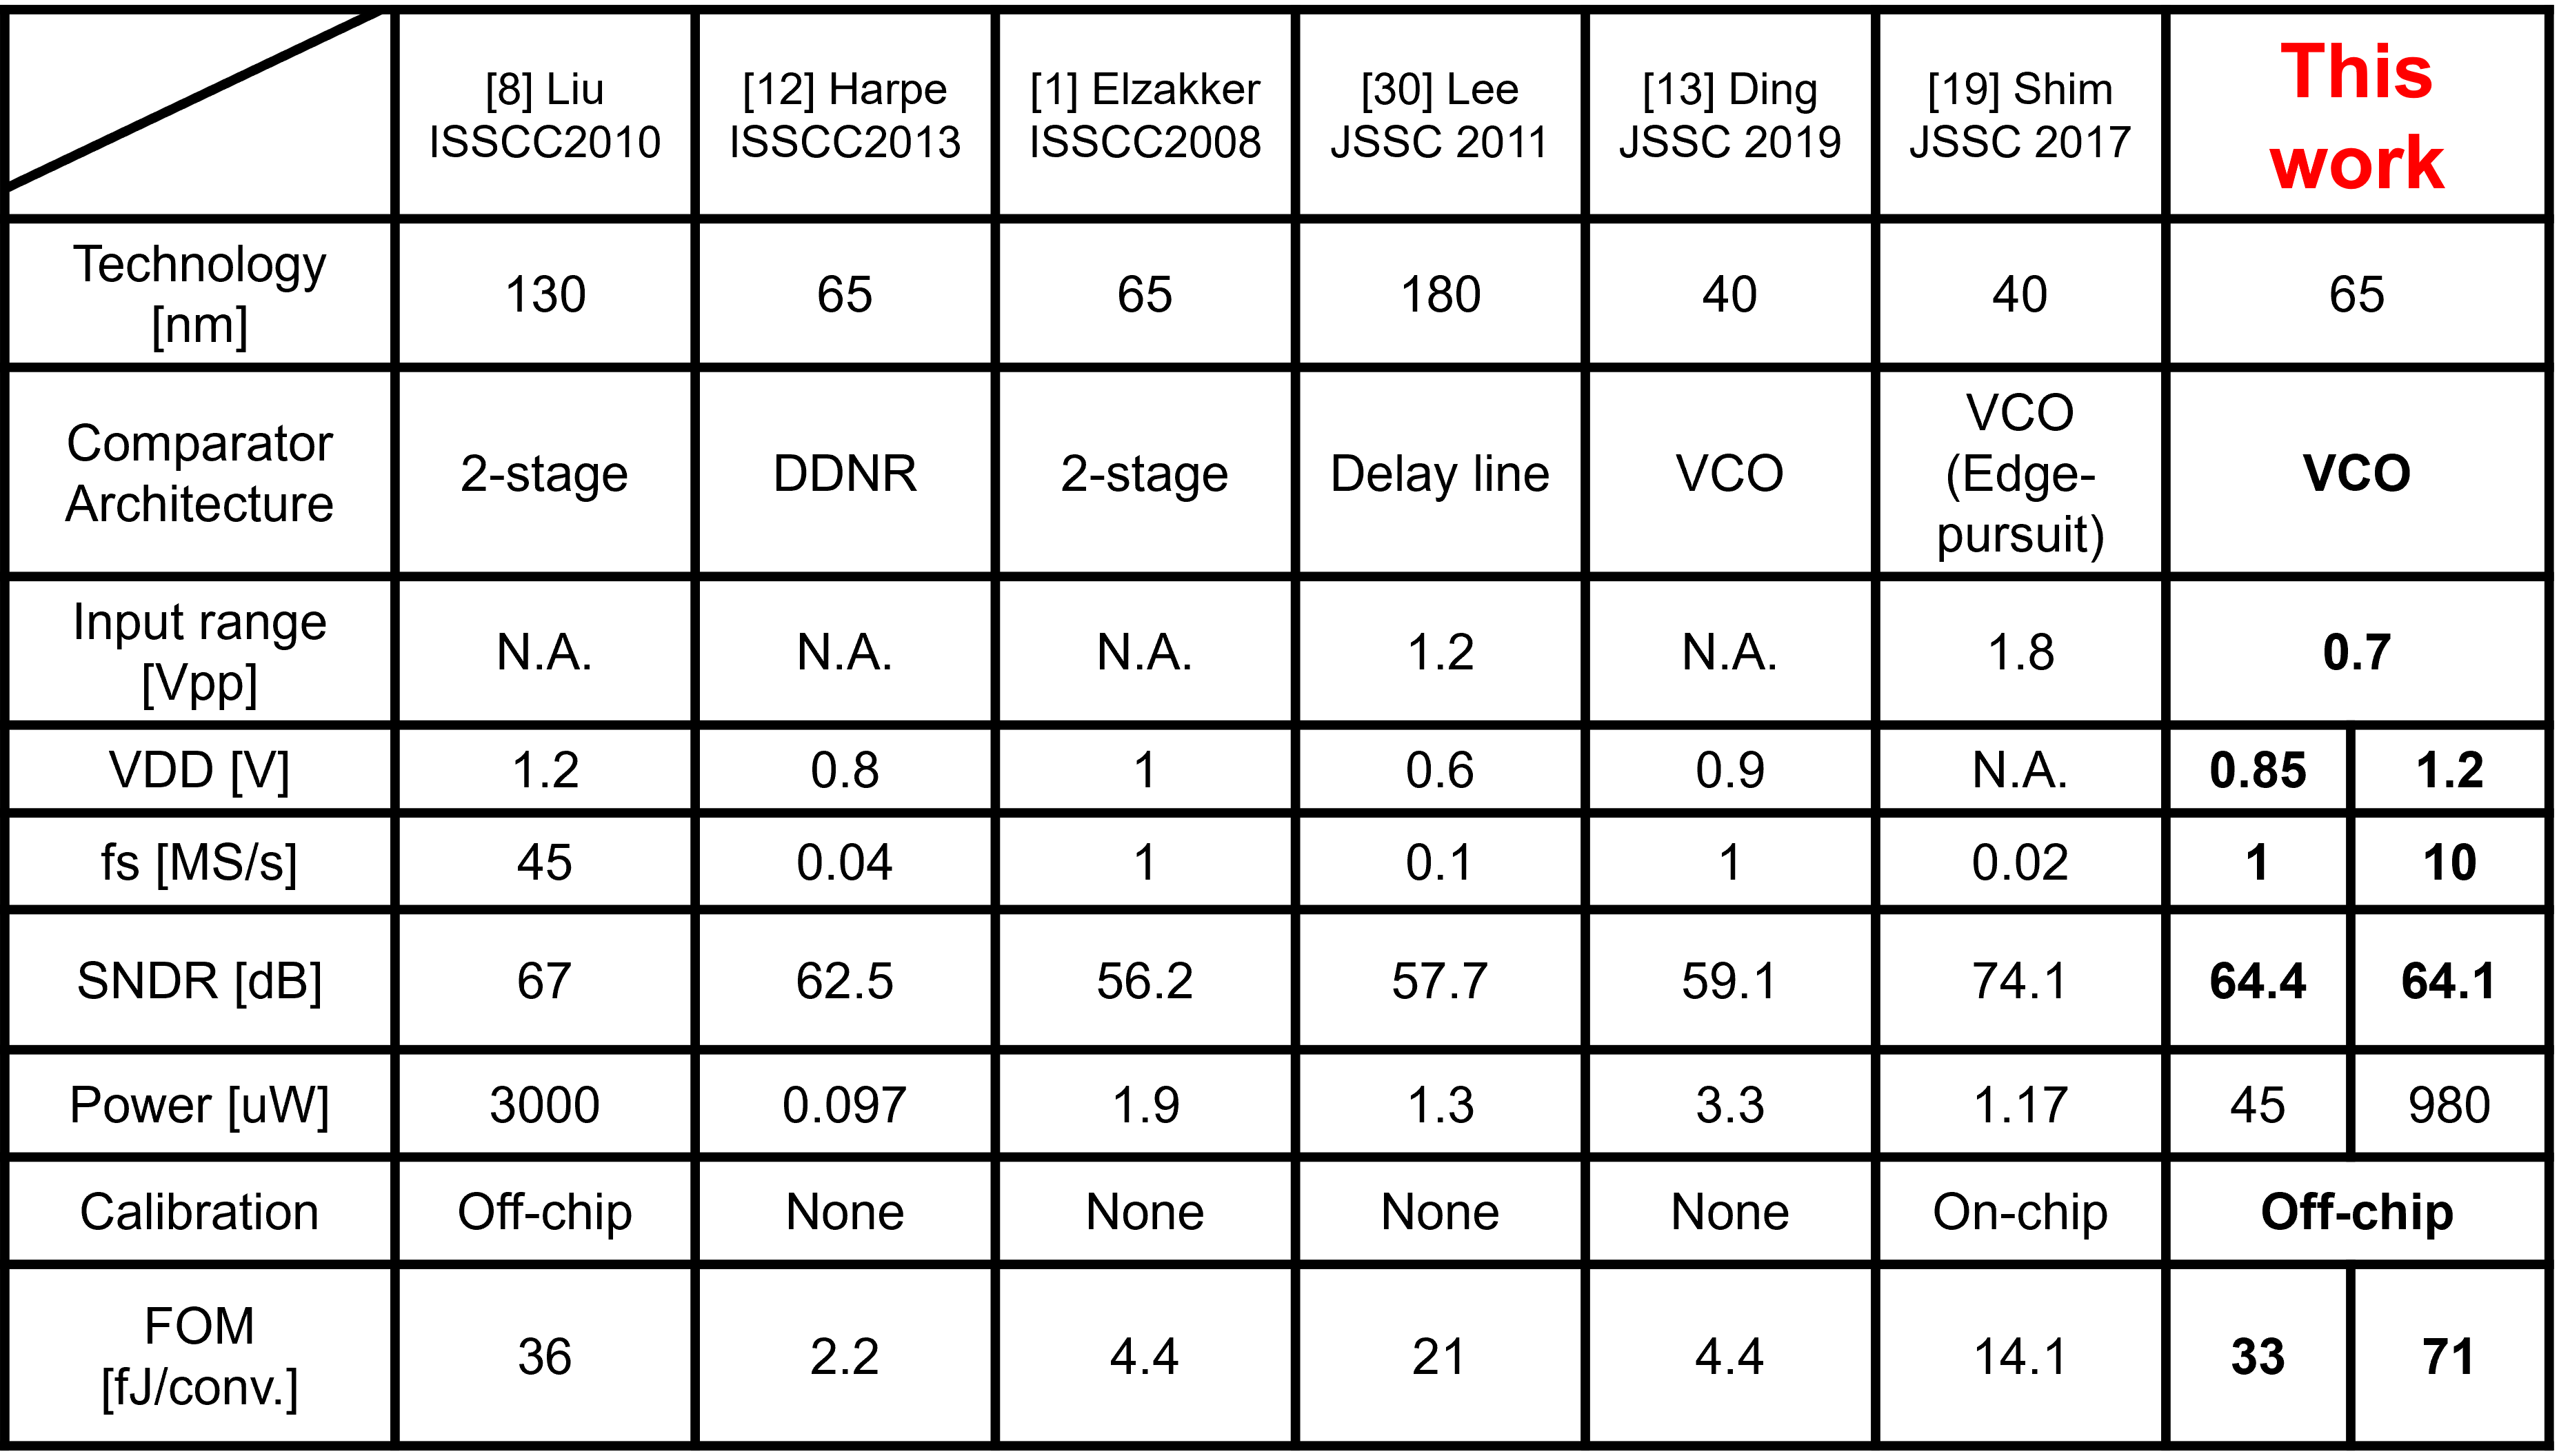
\includegraphics[width=0.5\textwidth]{figs/table.png}
  \captionsetup{font=footnotesize}
  \caption{\textbf{ADC}}
  \label{highlight}
\end{figure}

The SAR ADC was fabricated in 65-nm CMOS and Fig.8 shows the chip micrograph and a performance summary. 
Fig.9 shows a result of 16384-FFT before and after LMS calibration. The two FFT results were lead using the same raw data, but different bit weighting were used: weighting used in schematic and weighting derived via calibration. Therefore, noise situation is exactly the same. Even though no trimming to the comparator was carried out, fine noise performance was achieved. Even with LMS calibration, the SNDR was 66.4 dB, which was lower than expected. One reason for this is the poor IP3 performance of the signal generator which limits the input swing to 0.7Vpp.  The LMS engine requires about 26000 iterations to calibrate the radix and then perturbation injection can be stopped to save power. The power consumption shown in Fig.8 is measured when perturbation injection is off. If the LMS calibration engine was to be implemented on-chip and run background, we expect that the total power consumption will increase three-fold.
Finally, we plotted fs and fin versus SNDR performance in Fig.10. Since the VCO comparator is mostly digital, low voltage operation can be easily accomplished.  Thanks to the 
 
Fig.10 fin and fs versus SNDR plotted respectively

low-voltage operation of VCO based comparator, all of the measurements have been conducted with a single supply voltage of 0.85 V. At 1.2V supply, the ADC achieves the same SNDR performance and extends fs to 10MS/s. Although, we must be careful of the signal common-mode voltage (VCM), because this directly impacts the inverter’s gain bandwidth used in the VCO. When the VCM was increased beyond 0.5V, degradation in SNDR was observed.


\section{Conclusions}
To automatically reduce comparator noise at small dvin conditions, VCO comparator with eye-opening operation was introduced.  Even though the proposed VCO comparator was designed for 13b ADC, this comparator can be used for further resolution improvement by taking care of the jitter performance. Moreover, since this comparator is mainly based on inverters and other simple logic cells, benefits can be granted by process scaling. Furthermore, the characteristics can be surely analyzed using a well-known knowledge of oscillator and logic cells. 

\bibliographystyle{IEEEbib}
\bibliography{main}


\begin{IEEEbiography}
[{
\includegraphics[width=1in,height=1.25in,clip,keepaspectratio]{bio/1.jpg}}]{Kentaro Yoshioka}
received his BS, MS, Ph.D degrees from Keio University, Japan. Currently, he is an Assistant Professor at Keio University. He worked with Toshiba during 2014-2021, developing circuitry for WiFi and LiDAR SoCs. During 2017-2018, he had been a visiting scholar at Stanford University, exploring efficient machine learning hardware and algorithms. 

Currently, Dr. Yoshioka serves as a technical program member of Symp. VLSI circuits conference. Dr. Yoshioka was the recipient of ASP-DAC 2013 Special Feature Award,the A-SSCC 2012 Best Design Award, and 1st place winner of Kaggle Prostate Cancer Grade Assessment (PANDA) Challenge.
\end{IEEEbiography}

\end{document}
